
\chapter{Programmable Logic Controllers}

Every control system may be divided into three general sections: \textit{input} devices (sensors), \textit{controllers}, and \textit{output} devices (actuators).  The input devices sense what is happening in the process, the controller decides what to do about it, and the output devices manipulate the process to achieve the desired result.

A \textit{programmable logic controller} or \textit{PLC} is a general-purpose controller, applicable to many different types of process control applications.  The word ``programmable'' in its name reveals just why PLCs are so useful: the end-user is able to program, or instruct, the PLC to do virtually any control function imaginable.  Unlike PID loop controllers, which are special-purpose devices intended to perform a single type of control function, a PLC may be instructed to do almost anything with the signals it receives from input devices.  \index{Programmable Logic Controller}  \index{PLC}

PLCs were introduced to industry as electronic replacements for electromechanical relay controls.  In applications where relays typically control the starting and stopping of electric motors and other discrete output devices, the reliability of an electronic PLC meant fewer system failures and longer operating life.  The re-programmability of a PLC also meant changes could be implemented to the control system strategy must easier than with relay circuits, where re-wiring was the only way to alter the system's function.  Additionally, the computer-based nature of a PLC meant that process control data could now be communicated by the PLC over \textit{networks}, allowing process conditions to be monitored in distant locations, and by multiple operator stations.

The legacy of PLCs as relay-replacements is probably most evident in their traditional programming language: a graphical convention known as a \textit{Ladder Diagram}.  Ladder Diagram PLC programs resemble ladder-style electrical schematics, where vertical power ``rails'' convey control power to a set of parallel ``rung'' circuits containing switch contacts and relay coils.  A human being programming a PLC literally draws the diagram on the screen, using relay-contact symbols to represent instructions to read data bits in the PLC's memory, and relay-coil symbols to represent instructions writing data bits to the PLC's memory.  This style of programming was developed to make it easier for industrial electricians to adapt to the new technology of PLCs.  While Ladder Diagram programming definitely has limitations compared to other computer programming languages, it is relatively easy to learn and diagnose, which is why it remains popular as a PLC programming language today.  \index{Ladder Diagram}

Typical devices connecting to a PLC's inputs include hand switches, process switches, sensors, analog transmitters (4-20 mA), thermocouples, thermistors, and strain gauges.  Typical devices connecting to a PLC's outputs include electric lamps, solenoids, relay coils, motor contactors, analog final control elements (e.g. throttling control valves, variable-speed motor drives), and audible buzzers.  While PLCs were originally designed for discrete (on/off) control applications such as conveyor belt management, batch sequencing, and assembly line controls, modern PLCs are equally capable of inputting and outputting analog signals as well.  Thus, it is just as likely now to find a PLC performing PID loop control as it is to find a PLC turning discrete devices on and off.  \index{Contactor}




\filbreak
\section{PLC examples}

Programmable logic controllers are essentially nothing more than special-purpose, industrial computers.  As such, they are built far more ruggedly than an ordinary personal computer (PC), and designed to run extremely reliable operating system software\footnote{There are such things as \textit{soft PLCs}, which consist of special-purpose software running on an ordinary personal computer (PC) with some common operating system.  Soft PLCs enjoy the high speed and immense memory capacity of modern personal computers, but do not possess the same ruggedness either in hardware construction or in operating system design.  Their applications should be limited to non-critical controls where neither main process production nor safety would be jeopardized by a control system failure.}.  PLCs as a rule do not contain disk drives, cooling fans, or any other moving parts.  This is an intentional design decision, intended to maximize the reliability of the hardware in harsh industrial environments where the PLC chassis may be subjected to temperature extremes, vibration, humidity, and airborne particulates (dust, fibers, and/or fumes).

Large PLC systems consist of a rack into which circuit ``cards'' are plugged.  These cards include processors, input and output (I/O) points, communications ports, and other functions necessary to the operation of a complete PLC system.  Such ``modular'' PLCs may be configured differently according to the specific needs of the application.  Individual card failures are also easier to repair in a modular system, since only the failed card need be replaced, not all the cards or the whole card rack.  \index{I/O}

Small PLC systems consist of a monolithic ``brick'' containing all processor, I/O, and communication functions.  These PLCs are typically far less expensive than their modular cousins, but are also more limited in I/O capability and must be replaced as a whole in the event of failure.

\vskip 10pt

The following photographs show several examples of real PLC systems, some modular and some monolithic.  These selections are not comprehensive by any means, as there are many more manufacturers and models of PLC than those I have photographed.  They do, however, represent some of the more common brands and models in current (2010) industrial use.

\filbreak

The first photograph is of a Siemens (Texas Instruments) 505 series PLC, installed in a control panel of a municipal wastewater treatment plant.  This is an example of a modular PLC, with individual processor, I/O, and communication cards plugged into a rack.  Three racks appear in this photograph (two completely filled with cards, and the third only partially filled):  \index{Siemens 505 PLC}  \index{Texas Instruments 505 PLC}

$$\includegraphics[width=5in]{plc_001.eps}$$

The power supply and processor card for each rack is located on the left-hand end, with I/O cards plugged into slots in the rest of the rack.  Input devices such as switches and sensors connect by wire to terminals on \textit{input} cards, while output devices such as lamps, solenoids, and motor contactor coils connect by wire to terminals on \textit{output} cards.   \index{Contactor} 

One of the benefits of modular PLC construction is that I/O cards may be changed out as desired, altering the I/O configuration of the PLC as needed.  If, for example, the PLC needs to be configured to monitor a greater number of sensors, more input cards may be plugged into the rack and subsequently wired to those sensors.  Or, if the \textit{type} of sensor needs to be changed -- perhaps from a 24 volt DC sensor to one operating on 120 volts AC -- a different type of input card may be substituted to match the new sensor(s).

\vskip 10pt

In this particular application, the PLC is used to sequence the operation of self-cleaning ``trash racks'' used to screen large debris such as rags, sticks, and other non-degradable items from municipal wastewater prior to treatment.  These trash racks are actuated by electric motors, the captured debris scraped off and transported to a solid waste handling system.  The motion of the trash racks, the sensing of wastewater levels and pressures, and the monitoring of any human-operated override controls are all managed by these PLCs.  The programming of these PLCs involves timers, counters, sequencers, and other functions to properly manage the continuous operation of the trash racks.

\filbreak

The next photograph shows an Allen-Bradley (Rockwell) PLC-5 system, used to monitor and control the operation of a large natural gas compressor.  Two racks appear in this first photograph, with different types of I/O cards plugged into each rack:  \index{Rockwell PLC-5}  \index{Allen-Bradley PLC-5}

$$\includegraphics[width=5in]{plc_002.eps}$$

Like the Siemens 505 PLC seen previously, this Allen-Bradley PLC-5 system is fully modular and configurable.  The types and locations of the I/O cards inserted into the rack may be altered by appropriately skilled technicians to suit any desired application.  The programming of the PLC's processor card may also be altered if a change in the control strategy is desired for any reason.

In this particular application, the PLC is tasked with monitoring certain variables on the gas compressor unit, and taking corrective action if needed to keep the machine productive and safe.  The automatic control afforded by the PLC ensures safe and efficient start-ups, shut-downs, and handling of emergency events.  The networking and data-logging capability of the PLC ensures that critical data on the compressor unit may be viewed by the appropriate personnel.  For this particular compressor station, the data gets communicated from Washington state where the compressor is located all the way to Utah state where the main operations center is located.  Human operators in Utah are able to monitor the compressor's operating conditions and issue commands to the compressor over digital networks.

\vskip 10pt

Both the Siemens (formerly Texas Instruments) 505 and Allen-Bradley (Rockwell) PLC-5 systems are considered ``legacy'' PLC systems by modern standards, the two systems in the previous photographs being about 20 years old each.  It is not uncommon to find ``obsolete'' PLCs still in operation, though.  Given their extremely rugged construction and reliable design, these control systems may continue to operate without significant trouble for decades.

\filbreak

A newer model of PLC manufactured by Allen-Bradley is the SLC 500 series (often verbally referred to as the ``Slick 500''), which is also modular in design like the older PLC-5 system, although the racks and modules of the SLC 500 design are more compact.  The SLC 500 rack shown in the next photograph has 7 ``slots'' for processor and I/O cards to plug in to, numbered 0 through 6 (left to right):  \index{Rockwell SLC 500 PLC}  \index{Allen-Bradley SLC 500 PLC}

$$\includegraphics[width=5in]{plc_017.eps}$$

The first three slots of this particular SLC 500 rack (0, 1, and 2) are occupied by the processor card, an analog input card, and a discrete input card, respectively.  The slots 3 and 4 are empty (revealing the backplane circuit board and connectors for accepting new cards).  The slots 5 and 6 hold discrete output and analog output cards, respectively.

A feature visible on all cards in this system are numerous LED indicators, designed to show the status of each card.  The processor card has LED indicators for ``Run'' mode, ``Fault'' conditions, ``Force'' conditions (when either input or output bits have been forced into certain states by the human programmer for testing purposes), and communication network indicators.  Each discrete I/O card has indicator LEDs showing the on/off status of each I/O bit, and the analog card has a single LED showing that the card is powered.

\filbreak

A nine-slot SLC 500 system is shown in the next photograph, controlling a high-purity water treatment system for a biopharmaceuticals manufacturing facility.  As you can see in this photograph, not all slots in this particular rack are occupied by I/O cards either:

$$\includegraphics[height=5in]{plc_018.eps}$$

Some of the inputs to this PLC include water level switches, pressure switches, water flow meters, and conductivity meters (to measure the purity of the water, greater electrical conductivity indicating the presence of more dissolved minerals, which is undesirable in this particular process application).  In turn, the PLC controls the starting and stopping of water pumps and the switching of water valves to manage the water purification and storage processes.

\filbreak

A modern PLC manufactured by Siemens appears in this next photograph, an S7-300, which is a different design of modular PLC.  Instead of individual cards plugging into a rack, this modular PLC design uses individual modules plugging into each other on their sides to form a wider unit:  \index{Siemens S7-300 PLC}

$$\includegraphics[width=5in]{plc_003.eps}$$

A modern PLC manufactured by Allen-Bradley (Rockwell) is this ControlLogix 5000 system, shown in this photograph used to control a cereal manufacturing process.  The modular design of the ControlLogix 5000 system follows the more traditional scheme of individual cards plugged into a rack of fixed size:  \index{Rockwell ControlLogix 5000 PLC}  \index{Allen-Bradley ControlLogix 5000 PLC}

$$\includegraphics[width=5in]{plc_004.eps}$$

\filbreak

While the Siemens S7 and Rockwell ControlLogix PLC platforms represent large-scale, modular PLC systems, there exist much smaller PLCs available for a fraction of the cost.  Perhaps the least expensive PLC on the market at this time of writing is the Koyo ``CLICK'' PLC series, the processor module (with eight discrete input and six discrete output channels built in) shown in my hand (sold for 69 US dollars in the year 2010, and with free programming software!):  \index{Koyo CLICK PLC}  

$$\includegraphics[width=4in]{plc_005.eps}$$

This is a semi-modular PLC design, with a minimum of input/output (I/O) channels built into the processor module, but having the capacity to accept multiple I/O modules plugged in to the side, much like the Siemens S7-300 PLC.

\filbreak

Other semi-modular PLCs expand using I/O cards that plug in to the base unit not unlike traditional rack-based PLC systems.  The Koyo DirectLogic DL06 is a good example of this type of semi-modular PLC, the following photograph showing a model DL06 accepting a thermocouple input card in one of its four available card slots:  \index{Koyo DL06 PLC}

$$\includegraphics[width=4in]{plc_007.eps}$$

This photograph shows the PLC base unit with 20 discrete input channels and 16 discrete output channels, accepting an analog input card (this particular card is designed to input signals from thermocouples to measure up to four channels of temperature).

\filbreak

Some low-end PLCs are strictly monolithic, with no ability to accept additional I/O modules.  This General Electric Series One PLC (used to monitor a small-scale hydroelectric power generating station) is an example of a purely monolithic design, having no ``expansion'' slots to accept I/O cards:  \index{GE Series One PLC}

$$\includegraphics[width=4in]{plc_006.eps}$$

A disadvantage of monolithic PLC construction is that damaged I/O cannot be independently replaced.  If an I/O channel on one of these PLCs becomes damaged, the entire PLC must be replaced to fix the problem.  In a modular system, the damaged I/O card may simply be unplugged from the rack and replaced with a new I/O card.  Another disadvantage of monolithic PLCs is the inherently fixed nature of the I/O: the end-user cannot customize the I/O configuration to match the application.  For these reasons, monolithic PLCs are usually found on small-scale processes with few I/O channels and limited potential for expansion.







\filbreak
\section{Input/Output (I/O) capabilities}

Every programmable logic controller must have some means of receiving and interpreting signals from real-world sensors such as switches, and encoders, and also be able to effect control over real-world control elements such as solenoids, valves, and motors.  This is generally known as \textit{input/output}, or \textit{I/O}, capability.  Monolithic (``brick'') PLCs have a fixed amount of I/O capability built into the unit, while modular (``rack'') PLCs use individual circuit board ``cards'' to provide customized I/O capability.  \index{I/O}  

$$\includegraphics{plc_075.eps}$$

The advantages of using replaceable I/O cards instead of a monolithic PLC design are numerous.  First, and most obvious, is the fact that individual I/O cards may be easily replaced in the event of failure without having to replace the entire PLC.  Specific I/O cards may be chosen for custom applications, biasing toward discrete cards for applications using many on/off inputs and outputs, or biasing toward analog cards for applications using many 4-20 mA and similar signals.  Some PLCs even offer the feature of \textit{hot-swappable} cards, meaning each card may be removed and a new one inserted without de-energizing power to the PLC processor and rack.  Please note that one should not assume any system has hot-swappable cards, because if you attempt to change out a card ``live'' in a system without this feature, you run the risk of damaging the card and/or the rest of the unit it is plugged in to!  \index{Hot-swappable PLC I/O}  \index{I/O, hot-swappable}

\filbreak

Some PLCs have the ability to connect to processor-less remote racks filled with additional I/O cards or modules, thus providing a way to increase the number of I/O channels beyond the capacity of the base unit.  The connection from host PLC to remote I/O racks usually takes the form of a special digital network, which may span a great physical distance:  \index{Remote PLC I/O}  \index{I/O, remote}

$$\includegraphics{plc_008.eps}$$

An alternative scheme for system expansion is to network multiple PLCs together, where each PLC has its own dedicated rack and processor.  Through the use of communication instructions, one PLC may be programmed to read data from and/or write data to another PLC, effectively using the other PLC as an extension of its own I/O.  Although this method is more expensive than remote I/O (where the remote racks lack their own dedicated processors), it provides the capability of stand-alone control in the event the network connection between PLC processors becomes severed.

\vskip 10pt

Input/output capability for programmable logic controllers comes in three basic varieties: \textit{discrete}, \textit{analog}, and \textit{network}; each type discussed in a following subsection.







\filbreak
\subsection{Discrete I/O}

A ``discrete'' data point is one with only two states \textit{on} and \textit{off}.  Process switches, pushbutton switches, limit switches, and proximity switches are all examples of discrete sensing devices.  In order for a PLC to be aware of a discrete sensor's state, it must receive a signal from the sensor through a \textit{discrete input} channel.  Inside each discrete input module is (typically) a set of light-emitting diodes (LEDs) which will be energized when the corresponding sensing device turns on.  Light from each LED shines on a photo-sensitive device such as a phototransistor inside the module, which in turn activates a \textit{bit} (a single element of digital data) inside the PLC's memory.  This opto-coupled arrangement makes each input channel of a PLC rather rugged, capable of isolating the sensitive computer circuitry of the PLC from transient voltage ``spikes'' and other electrical phenomena capable of causing damage:  \index{Bit}  \index{I/O, discrete (PLC)}

$$\includegraphics{plc_073.eps}$$

The internal schematic diagram for a discrete input module (``card'') shown above reveals the componentry typical for a single input channel on that card.  Each input channel has its own optocoupler, writing to its own unique memory register bit inside the PLC's memory.  Discrete input cards for PLCs typically have 4, 8, 16, or 32 channels.

\filbreak

Indicator lamps, solenoid valves, and motor starters (assemblies consisting of contactors and overload protection devices) are all examples of discrete control devices.  In a manner similar to discrete inputs, a PLC connects to any number of different discrete final control devices through a \textit{discrete output channel}\footnote{I/O ``channels'' are often referred to as ``points'' in industry lingo.  Thus, a ``32-point input card'' refers to an input circuit with 32 separate channels through which to receive signals from on/off switches and sensors.}.  Discrete output modules typically use the same form of opto-isolation to allow the PLC's computer circuitry to send electrical power to loads: the internal PLC circuitry driving an LED which then activates some form of photosensitive switching device.  Alternatively, small electromechanical relays may be used in lieu of opto-isolating semiconductor switching elements such as transistors (DC) or TRIACs (AC):

$$\includegraphics{plc_074.eps}$$

As with the schematic diagram for a discrete input module shown previously, the schematic diagram shown here for a discrete output module reveals the componentry typical for a single channel on that card.  Each output channel has its own optocoupler, driven by its own unique memory register bit inside the PLC's memory.  Discrete output cards for PLCs also typically have 4, 8, 16, or 32 channels.

\vskip 10pt

\filbreak

An important concept to master when working with DC discrete I/O is the distinction between \textit{current-sourcing} and \textit{current-sinking} devices.  The terms ``sourcing'' and ``sinking'' refer to the direction of current (as denoted by conventional flow notation) into or out of a device's control wire\footnote{By ``control wire,'' I mean the single conductor connecting the I/O card channel to the field device, as opposed to conductors directly common with either the positive or negative lead of the voltage source.  If you focus your attention on this one wire, noting the direction of conventional-flow current through it, the task of determining whether a device is sourcing or sinking current becomes much simpler.}.  A device sending (conventional flow) current out of its control terminal to some other device(s) is said to be \textit{sourcing} current, while a device accepting (conventional flow) current into its control terminal is said to be \textit{sinking} current.  \index{Sourcing current}  \index{Sinking current}  \index{Current sourcing}  \index{Current sinking}

\filbreak

To illustrate, the following illustration shows a PLC output channel is \textit{sourcing} current to an indicator lamp, which is \textit{sinking} current to ground:

$$\includegraphics{plc_009.eps}$$

These terms really only make sense when electric current is viewed from the perspective of conventional flow, where the positive terminal of the DC power supply is envisioned to be the ``source'' of the current, with current finding its way ``down'' to ground (the negative terminal of the DC power supply).  In every circuit formed by the output channel of a PLC driving a discrete control device, or by a discrete sensing device driving an input channel on a PLC, one element in the circuit must be sourcing current while the other is sinking current.

An engineering colleague of mine has a charming way to describe sourcing and sinking: \textit{blowing} and \textit{sucking}.  A device that sources current to another ``blows'' current toward the other device.  A device that sinks current ``sucks'' current from the other device.  Many students seem to find these terms helpful in first mastering the distinction between sourcing and sinking despite (or perhaps because of!) their informal nature.

\filbreak

If the discrete device connecting to the PLC is not polarity-sensitive, either type of PLC I/O module will suffice.  For example, the following diagrams show a mechanical limit switch connecting to a sinking PLC input and to a sourcing PLC input:

$$\includegraphics{plc_010.eps}$$

$$\includegraphics{plc_011.eps}$$

Note the differences in polarity and labeling between the sinking card's common terminal and the sourcing card's common terminal.  On the ``sinking'' card, the input channel terminal is positive while the common (``Com'') terminal is negative.  On the ``sourcing'' card, the input channel terminal is negative while the common (``VDC'') terminal is positive. 

\filbreak

Some discrete sensing devices \textit{are} polarity-sensitive, such as electronic proximity sensors containing transistor outputs.  A ``sourcing'' proximity switch can only interface with a ``sinking'' PLC input channel, and vice-versa:  \index{Sourcing current}  \index{Sinking current}  \index{Current sourcing}  \index{Current sinking}

$$\includegraphics{plc_012.eps}$$

In all cases, the ``sourcing'' device sends current \textit{out of} its signal terminal while the ``sinking'' device takes current \textit{into} its signal terminal.

\filbreak

Two photographs of a DC (sinking) discrete input module for an Allen-Bradley model SLC 500 PLC are shown here: one with the plastic cover closed over the connection terminals, and the other with the plastic cover opened up for viewing the terminals.  A legend on the inside of the cover shows the purpose of each screw terminal: eight input channels (numbered 0 through 7) and two redundant ``DC Com'' terminals for the negative pole of the DC power supply to connect:

$$\includegraphics[height=3in]{plc_013.eps} \hskip 30pt \includegraphics[height=3in]{plc_014.eps}$$

A standard feature found on practically every PLC discrete I/O module is a set of LED indicators visually indicating the status of each bit (discrete channel).  On the SLC 500 module, the LEDs appear as a cluster of eight numbered squares near the top of the module.

A photograph of discrete output terminals on another brand of PLC (a Koyo model DL06) shows somewhat different labeling:

$$\includegraphics[width=5in]{plc_015.eps}$$

Here, each output channel terminal is designated with a letter/number code beginning with the letter ``Y''.  Several ``common'' terminals labeled with ``C'' codes service clusters of output channels.  In this particular case, each ``common'' terminal is common only to four output channels.  With sixteen total output channels on this PLC, this means there are four different ``common'' terminals.  While this may seem somewhat strange (why not just have one ``common'' terminal for all sixteen output channels?), it more readily permits different DC power supplies to service different sets of output channels.

\vskip 10pt

Electrical polarity is not an issue with AC discrete I/O, since the polarity of AC reverses periodically anyway.  However, there is still the matter of whether the ``common'' terminal on a discrete PLC module will connect to the \textit{neutral} (grounded) or \textit{hot} (ungrounded) AC power conductor.

The next photograph shows a discrete AC output module for an Allen-Bradley SLC 500 PLC, using TRIACs as power switching devices rather than transistors as is customary with DC discrete output modules:

$$\includegraphics[height=4in]{plc_021.eps}$$

This particular eight-channel module provides two sets of TRIACs for switching power to AC loads, each set of four TRIACs receiving AC power from a ``hot'' terminal (VAC 1 or VAC 2), the other side of the load device being connected to the ``neutral'' (grounded) conductor of the AC power source.

\vskip 10pt

Fortunately, the hardware reference manual supplied by the manufacturer of every PLC shows diagrams illustrating how to connect discrete input and output channels to field devices.  One should always consult these diagrams before connecting devices to the I/O points of a PLC!








\filbreak
\subsection{Analog I/O}

In the early days of programmable logic controllers, processor speed and memory were too limited to support anything but discrete (on/off) control functions.  Consequently, the only I/O capability found on early PLCs were discrete in nature\footnote{Some modern PLCs such as the Koyo ``CLICK'' are also discrete-only.  Analog I/O and processing is significantly more complex to engineer and more expensive to manufacture than discrete control, and so low-end PLCs are more likely to lack analog capability.}.  Modern PLC technology, though, is powerful enough to support the measurement, processing, and output of analog (continuously variable) signals.  \index{I/O, analog (PLC)}

All PLCs are digital devices at heart.  Thus, in order to interface with an analog sensor or control device, some ``translation'' is necessary between the analog and digital worlds.  Inside every analog input module is an \textit{ADC}, or \textit{Analog-to-Digital Converter}, circuit designed to convert an analog electrical signal into a multi-bit binary word.  Conversely, every analog output module contains a \textit{DAC}, or \textit{Digital-to-Analog Converter}, circuit to convert the PLC's digital command words into analog electrical quantities.  \index{Analog-to-digital converter}  \index{ADC}  \index{Digital-to-analog converter}  \index{DAC}

Analog I/O is commonly available for modular PLCs for many different analog signal types, including:

\begin{itemize}
\item Voltage (0 to 10 volt, 0 to 5 volt)
\item Current (0 to 20 mA, 4 to 20 mA)
\item Thermocouple (millivoltage)
\item RTD (millivoltage)
\item Strain gauge (millivoltage)
\end{itemize}

\filbreak

The following photographs show two analog I/O cards for an Allen-Bradley SLC 500 modular PLC system, an analog input card and an analog output card.  Labels on the terminal cover doors indicate screw terminal assignments:

$$\includegraphics[height=4in]{plc_019.eps} \hskip 30pt \includegraphics[height=4in]{plc_020.eps}$$










\filbreak
\subsection{Network I/O}

Many different digital network standards exist for PLCs to communicate with, from PLC to PLC and between PLCs and field devices.  One of the earliest digital protocols developed for PLC communication was \textit{Modbus}, originally for the Modicon brand of PLC.  Modbus was adopted by other PLC and industrial device manufacturers as a \textit{de facto} standard\footnote{A ``de facto'' standard is one arising naturally out of legacy rather than by an premeditated agreement between parties.  Modbus and Profibus networks are considered ``de facto'' standards because those networks were designed, built, and marketed by pioneering firms prior to their acceptance as standards for others to conform to.  In Latin, \textit{de facto} means ``from the fact,'' which in this case refers to the fact of pre-existence: a standard agreed upon to conform to something already in popular use.  By contrast, a standard intentionally agreed upon before its physical realization is a \textit{de jure} standard (Latin for ``from the law'').  FOUNDATION Fieldbus is an example of a \textit{de jure} standard, where a committee arrives at a consensus for a network design and specifications prior to that network being built and marketed by any firm.}, and remains perhaps the most universal digital protocol available for industrial digital devices today. \index{Modbus}  \index{I/O, network (PLC)}

Another digital network standard developed by a particular manufacturer and later adopted as a \textit{de facto} standard is \textit{Profibus}, originally developed by Siemens.  \index{Profibus}

For more information on networking standards used in PLC systems, refer to the ``Digital electronic instrumentation'' chapter, specifically sections on specific network standards such as Modbus and Profibus.










\filbreak
\section{Logic programming}

Although it seems each model of PLC has its own idiosyncratic standard for programming, there does exist an international standard for controller programming that most PLC manufacturers at least attempt to conform to.  This is the IEC 61131-3 standard, which will be the standard presented in this chapter.  \index{IEC standard 61131-3 (PLC programming languages)}

One should take solace in the fact that despite differences in the details of PLC programming from one manufacturer to another and from one model to another, the basic principles are largely the same.  There exist much greater disparities between different general-purpose programming languages (e.g. C/C++, BASIC, FORTRAN, Pascal, Java, Ada, etc.) than between the programming languages supported by different PLCs, and this fact does not prevent computer programmers from being ``multilingual.''  I have personally written and/or analyzed programs for over a half-dozen different manufacturers of PLCs (Allen-Bradley, Siemens, Square D, Koyo, Fanuc, Moore Products APACS and QUADLOG, and Modicon), with multiple PLC models within most of those brands, and I can tell you the differences in programming conventions are largely insignificant.  After learning how to program one model of PLC, it is quite easy to adapt to programming other makes and models of PLC.  If you are learning to program a particular PLC that does not exactly conform to the IEC 61131-3 standard, you will still be able to apply every single principle discussed in this chapter -- the fundamental concepts are truly that universal.

The IEC 61131-3 standard specifies five distinct forms of programming language for industrial controllers:

\begin{itemize}
\item Ladder Diagram (LD)
\item Structured Text (ST)
\item Instruction List (IL)
\item Function Block Diagram (FBD)
\item Sequential Function Chart (SFC)
\end{itemize}

Not all programmable logic controllers support all five language types, but nearly all of them support Ladder Diagram (LD), which will be the primary focus of this book.

Programming languages for many industrial devices are limited by design.  One reason for this is \textit{simplicity}: any programming language simple enough in structure for someone with no formal computer programming knowledge to understand is going to be limited in its capabilities.  Another reason for programming limitations is \textit{safety}: the more flexible and unbounded a programming language is, the more potential there will be to unintentionally create complicated ``run-time'' errors when programming.  The ISA safety standard number 84 classifies industrial programming languages as either \textit{Fixed Programming Languages} (FPL), \textit{Limited Variability Languages} (LVL), or \textit{Full Variability Languages} (FVL).  Ladder Diagram and Function Block Diagram programming are both considered to be ``limited variability'' languages, whereas Instruction List (and traditional computer programming languages such as C/C++, FORTRAN, BASIC, etc.) are considered ``full variability'' languages with all the attendant potential for complex errors.  \index{ISA 84}  \index{Fixed Programming Language (FPL)}  \index{Limited Variability Language (LVL)}  \index{Full Variability Language (FVL)}

% ADD: note the extreme importance of properly documenting control programs, and also maintaining backup copies in case of data loss






\filbreak
\subsection{Relating I/O status to virtual elements}

Perhaps the most important yet elusive concept to grasp when learning to program PLCs is the relationship between the electrical status of the PLC's I/O points and the status of variables and other ``elements'' in its programming.  This is especially true for Ladder Diagram (LD) programming, where the program itself resembles an electrical diagram.  Making the mental connection between the ``real'' world of the switches, contactors, and other electrical devices connected to the PLC and the ``imaginary'' world of the PLC's program consisting of virtual contacts and relay ``coils'' is most fundamental.

The first fundamental rule one should keep in mind when examining a Ladder Diagram PLC program is that \textbf{each virtual contact shown in the program \textit{actuates} whenever it reads a ``1'' state in its respective bit and will be \textit{at rest} whenever it reads a ``0'' state in its respective bit} (in the PLC's memory).  If the contact is a normally-open (NO) type, it will open when its bit is 0 and close when its bit is 1.  If the contact is a normally-closed (NC) type, it will close when its bit is 0 and open when its bit is 1.  A 0 bit state causes the contact to be in its ``normal'' (resting) condition, while a 1 bit state \textit{actuates} the contact, forcing it into its non-normal (actuated) state.   \index{Normal state of a PLC program contact}

Another rule to remember when examining a Ladder Diagram PLC program is that the programming software offers \textit{color highlighting}\footnote{It should be noted that in some situations the programming software will fail to color the contacts properly, especially if their status changes too quickly for the software communication link to keep up, and/or if the bit(s) change state multiple times within one scan of the program.  However, for simple programs and situations, this rule holds true and is a great help to beginning programmers as they learn the relationship between real-world conditions and conditions within the PLC's ``virtual'' world.} to display the virtual status of each program element: \textbf{a colored contact is \textit{closed}, while an un-colored contact is \textit{open}}.  While the presence or absence of a ``slash'' symbol marks the \textit{normal} status of a contact, its live color highlighting shown by PLC programming software reveals the ``conductive'' status of the elements \textit{in real time}.

The following table shows how the two types of contacts in a PLC's Ladder Diagram program respond to bit states, using red coloring to signify each contact's virtual conductivity:

$$\includegraphics{plc_065.eps}$$

Just as a pressure switch's contacts are actuated by a high pressure condition, and a level switch's contacts are actuated by a high level condition, and a temperature switch's contacts are actuated by a high temperature condition, so a PLC's virtual contact is actuated by a high \textit{bit} condition (1).  In the context of any switch, an \textit{actuated} condition is the opposite of its \textit{normal} (resting) condition.

\filbreak

The following simplified\footnote{The electrical wiring shown in this diagram is incomplete, with the ``Common'' terminal shown unconnected for simplicity's sake.} illustration shows a small PLC with two of its discrete input channels electrically energized, causing those two bits to have ``1'' statuses.  The color-highlighted contacts in the programming editor software's display shows a collection of contacts addressed to those input bits in various states (colored = closed ; un-colored = open).  As you can see, every contact addressed to a ``set'' bit (1) is in its actuated state, while every contact addressed to a ``cleared'' bit (0) is in its normal state:

$$\includegraphics{plc_064.eps}$$

Remember that a \textit{colored} contact is a \textit{closed} contact.  The contacts appearing as colored are either normally-closed contacts with ``0'' bit states, or normally-open contacts with ``1'' bit states.  It is the combination of bit state and contact type (NO vs. NC) that determines whether the virtual contact will be open (un-colored) or closed (colored) at any given time.  Correspondingly, it is a combination of colored highlighting and virtual contact type that indicates the real-world energization status of a particular PLC input at any given time.

\filbreak

In my teaching experience, the main problem students have comprehending PLC Ladder Diagram programs is that they over-simplify and try to directly associate real-world switches connected to the PLC with their respective contact instructions inside the PLC program.  Students mistakenly think the real-world switch connecting to the PLC and the respective virtual switch contact inside the PLC program are one and the same, when this is not the case at all.  Rather, the real-world switch sends power to the PLC input, \textit{which in turn \underbar{controls} the state of the virtual contact(s) programmed into the PLC.}  Specifically, I see students routinely fall into the following mis-conceptions:

\begin{itemize}
\item Students mistakenly think the contact instruction type (NO vs. NC) needs to match that of its associated real-world switch
\item Students mistakenly think color highlighting of a contact instruction is equivalent to the electrical status of its associated real-world PLC input
\item Students mistakenly think a closed real-world switch must result in a closed contact instruction in the live PLC program
\end{itemize}

To clarify, here are the fundamental rules one should keep in mind when interpreting contact instructions in Ladder Diagram PLC programs:

\begin{itemize}
\item \textbf{Each input bit in the PLC's memory will be a ``1'' when its input channel is powered, and will be a ``0'' when its input channel is unpowered}
\item \textbf{Each virtual contact shown in the program \textit{actuates} whenever it reads a ``1'' state in its respective bit, and will be \textit{at rest} whenever it reads a ``0'' state in its respective bit}
\item \textbf{A colored contact is \textit{closed} (passes virtual power in the PLC program), while an un-colored contact is \textit{open} (blocks virtual power in the PLC program)}
\end{itemize}

In trying to understand PLC Ladder Diagram programs, the importance of these rules cannot be overemphasized.  The truth of the matter is a causal chain -- rather than a direct equivalence -- between the real-world switch and the contact instruction status.  The real-world switch controls whether or not electrical power reaches the PLC input channel, which in turn controls whether the input register bit will be a ``1'' or a ``0'', which in turn controls whether the contact instruction will actuated or at rest.  Virtual contacts inside the PLC program are thus \textit{controlled} by their corresponding real-world switches, rather than simply being \textit{identical} to their real-world counterparts as novices tend to assume.  Following these rules, we see that normally-open (NO) contact instructions will mimic what their real-world switches are doing, while normally-closed (NC) contact instructions will act opposite of their real-world counterparts.

% ADD: show relay analogy, where each PLC input is a special coil electrically energized by a real-world switch.  Show relay circuit first, then follow with modified diagram showing how the PLC implements the same logic.

\vskip 10pt

The color highlighting of \textit{coil} instructions in a Ladder Diagram PLC program follows similar rules.  A coil will be ``on'' (colored) when all contact instructions prior to it are closed (colored).  A colored coil writes a ``1'' to its respective bit in memory, while an un-colored coil instruction writes a ``0'' to its respective bit in memory.  If these bits are associated with real-world discrete output channels on the PLC, their states will control the real-world energization of devices electrically connected to those channels.

\filbreak

To further illuminate these fundamental concepts, we will examine the operation of a simple PLC system designed to energize a warning lamp in the event that a process vessel experiences a high fluid pressure.  The PLC's task is to energize a warning lamp if the process vessel pressure ever exceeds 270 PSI, and keep that warning lamp energized even if the pressure falls below the trip point of 270 PSI.  This way, operators will be alerted to both \textit{past} and \textit{present} process vessel overpressure events.

120 volt AC ``line'' power (L1 and L2) provides electrical energy for the PLC to operate, as well as signal potential for the input switches and power for the warning lamp.  Two switches connect to the input of this PLC: one normally-open pushbutton switch acting as the alarm reset (pressing this switch ``unlatches'' the alarm lamp) and one normally-open pressure switch acting as the sensing element for high process vessel pressure: 

$$\includegraphics{plc_055.eps}$$

The reset pushbutton connects to discrete input \texttt{X1} of the PLC, while the pressure switch connects to discrete input \texttt{X4}.  The warning lamp connects to discrete output \texttt{Y5}.  Red indicator LEDs next to each I/O terminal visually indicate the electrical status of the I/O points, while red-shaded highlighting shows the \textit{virtual power}\footnote{For a PLC program contact, the shading represents virtual ``conductivity.''  For a PLC program coil, the shading represents a set (1) bit.} status of the ``contacts'' and ``coils'' in the PLC's program, displayed on the screen of a personal computer connected to the PLC through a programming cable.

With no one pressing the reset pushbutton, that switch will be in its normal status, which for a ``normally-open'' switch is open.  Likewise with the pressure switch: with process pressure less than the trip point of 270 PSI, the pressure switch will also be in its normal status, which for a ``normally-open'' switch is open.  Since neither switch is conducting electricity right now, neither discrete input \texttt{X1} nor \texttt{X4} will be energized.  This means the ``virtual'' contacts inside the PLC program will likewise be in their own normal states.  Thus, any virtual contact drawn as a normally-open will be open (not passing virtual power), and any virtual contact drawn as a normally-closed (a diagonal slash mark through the contact symbol) will be closed.  This is why the two normally-open virtual contacts \texttt{X4} and \texttt{Y5} have no highlighting, but the normally-closed virtual contact \texttt{X1} does -- the colored highlighting representing the ability to pass virtual power.

\vskip 10pt

\filbreak

If the process vessel experiences a high pressure ($>$ 270 PSI), the pressure switch will actuate, closing its normally-open contact.  This will energize input \texttt{X4} on the PLC, which will ``close'' the virtual contact \texttt{X4} in the ladder program.  This sends virtual power to the virtual ``coil'' \texttt{Y5}, which in turn latches itself on through virtual contact \texttt{Y5}\footnote{It is worth noting the legitimacy of referencing virtual contacts to output bits (e.g. contact \texttt{Y5}), and not just to input bits.  A ``virtual contact'' inside a PLC program is nothing more than an instruction to the PLC's processor to \textit{read} the status of a bit in memory.  It matters not whether that bit is associated with a physical input channel, a physical output channel, or some abstract bit in the PLC's memory.  It would, however, be wrong to associate a virtual coil with an input bit, as coil instructions \textit{write} bit values to memory, and input bits are supposed to be controlled solely by the energization states of their physical input channels.} and also energizes the real discrete output \texttt{Y5} to energize the warning lamp:

$$\includegraphics{plc_056.eps}$$



\filbreak

If now the process pressure falls below 270 PSI, the pressure switch will return to its normal state (open), thus de-energizing discrete input \texttt{X4} on the PLC.  Because of the latching contact \texttt{Y5} in the PLC's program, however, output \texttt{Y5} remains on to keep the warning lamp in its energized state:

$$\includegraphics{plc_057.eps}$$

Thus, the \texttt{Y5} contact performs a \textit{seal-in} function to keep the \texttt{Y5} bit set (1) even after the high-pressure condition clears.  This is precisely the same concept as the ``seal-in'' auxiliary contact on a hard-wired motor starter circuit, where the electromechanical contactor keeps itself energized after the ``Start'' pushbutton switch has been released.  \index{Seal-in contact}  \index{Auxiliary contact}  \index{Contactor}

\filbreak

The only way for a human operator to re-set the warning lamp is to press the pushbutton.  This will have the effect of energizing input \texttt{X1} on the PLC, thus opening virtual contact \texttt{X1} (normally-closed) in the program, thus interrupting virtual power to the virtual coil \texttt{Y5}, thus powering down the warning lamp and un-latching virtual power in the program:

$$\includegraphics{plc_058.eps}$$

% ADD: possibly show the exact same logic sequence in function-block programming (AND, OR, and NOT gates in the PC display instead of contacts and coils)







%\filbreak
%\subsection{PLC scan cycles}

% Allen-Bradley SLC 500 & MicroLogix:
%%  (1) Read inputs
%%  (2) Execute program
%%  (3) Write outputs
%%  (4) Communications
%%  (5) Overhead tasks (memory management)

% Siemens S7-200:
%%  (1) Read inputs
%%  (2) Execute program
%%  (3) Communications
%%  (4) CPU self-diagnostics
%%  (5) Write outputs

% Koyo ``CLICK'':
%%  (1) Read inputs
%%  (2) Service peripherals
%%  (3) Update special registers
%%  (4) Execute program
%%  (5) Write outputs
%%  (6) CPU self-diagnostics

% ADD: discuss ``immediate'' contact and coil (read and write) instructions





\filbreak
\subsection{Memory maps and I/O addressing}

A wise PLC programmer once told me that the first thing any aspiring programmer should learn about the PLC they intend to program is how the digital memory of that PLC is organized.  This is sage advice for any programmer, especially on systems where memory is limited, and/or where I/O has a fixed association with certain locations in the system's memory.  Virtually every microprocessor-based control system comes with a published \textit{memory map} showing the organization of its limited memory: how much is available for certain functions, which addresses are linked to which I/O points, how different locations in memory are to be referenced by the programmer.

Discrete input and output channels on a PLC correspond to individual \textit{bits} in the PLC's memory array.  Similarly, analog input and output channels on a PLC correspond to multi-bit \textit{words} (contiguous blocks of bits) in the PLC's memory.  The association between I/O points and memory locations is by no means standardized between different PLC manufacturers, or even between different PLC models designed by the same manufacturer.  This makes it difficult to write a general tutorial on PLC addressing, and so my ultimate advice is to consult the engineering references for the PLC system you intend to program.  

The most common brand of PLC in use in the United States at the time of this writing (2010) is Allen-Bradley (Rockwell), which happens to use a unique form of I/O addressing\footnote{The most modern Allen-Bradley PLCs have all but done away with fixed-location I/O addressing, opting instead for \textit{tag name} based I/O addressing.  However, enough legacy Allen-Bradley PLC systems still exist in industry to warrant coverage of these addressing conventions.} students tend to find confusing.  For these two reasons (popularity and confusion), I will focus on Allen-Bradley addressing conventions for the bulk of this section.

\filbreak

The following table shows a partial memory map for an Allen-Bradley SLC 500 PLC\footnote{Also called the \textit{data table}, this map shows the addressing of memory areas reserved for programs entered by the user.  Other areas of memory exist within the SLC 500 processor, but these other areas are inaccessible to the technician writing PLC programs.}: \index{Memory map}

% No blank lines allowed between lines of an \halign structure!
% I use comments (%) instead, so that TeX doesn't choke.

$$\vbox{\offinterlineskip
\halign{\strut
\vrule \quad\hfil # \ \hfil & 
\vrule \quad\hfil # \ \hfil & 
\vrule \quad\hfil # \ \hfil \vrule \cr
\noalign{\hrule}
%
% First row
\textbf{File number} & \textbf{File type} & \textbf{Logical address range} \cr
%
\noalign{\hrule}
%
% Another row
0 & Output image & \texttt{O:0} to \texttt{O:30} \cr
%
\noalign{\hrule}
%
% Another row
1 & Input image & \texttt{I:0} to \texttt{I:30} \cr
%
\noalign{\hrule}
%
% Another row
2 & Status & \texttt{S:0} to \texttt{S:}$n$ \cr
%
\noalign{\hrule}
%
% Another row
3 & Binary & \texttt{B3:0} to \texttt{B3:255} \cr
%
\noalign{\hrule}
%
% Another row
4 & Timers & \texttt{T4:0} to \texttt{T4:255} \cr
%
\noalign{\hrule}
%
% Another row
5 & Counters & \texttt{C5:0} to \texttt{C5:255} \cr
%
\noalign{\hrule}
%
% Another row
6 & Control & \texttt{R6:0} to \texttt{R6:255} \cr
%
\noalign{\hrule}
%
% Another row
7 & Integer & \texttt{N7:0} to \texttt{N7:255} \cr
%
\noalign{\hrule}
%
% Another row
8 & Floating-point & \texttt{F8:0} to \texttt{F8:255} \cr
%
\noalign{\hrule}
%
% Another row
9 & Network & \texttt{x9:0} to \texttt{x9:255} \cr
%
\noalign{\hrule}
%
% Another row
10 through 255 & User defined & \texttt{x10:0} to \texttt{x255:255} \cr
%
\noalign{\hrule}
} % End of \halign 
}$$ % End of \vbox

Note that Allen-Bradley's use of the word ``file'' differs from personal computer parlance.  In the SLC 500 controller, a ``file'' is a block of random-access memory used to store a particular type of data.  By contrast, a ``file'' in a personal computer is a contiguous collection of data bits with collective meaning (e.g. a word processing file or a spreadsheet file), usually stored on the computer's hard disk drive.  Within each of the Allen-Bradley PLC's ``files'' are multiple ``elements,'' each element consisting of a set of bits (8, 16, 24, or 32) representing data.  Elements are addressed by number following the colon after the file designator, and individual bits within each element addressed by a number following a slash mark.  For example, the first bit (bit 0) of the second element in file 3 (Binary) would be addressed as \texttt{B3:2/0}.  

In Allen-Bradley PLCs such as the SLC 500 and PLC-5 models, files 0, 1, and 2 are exclusively reserved for discrete outputs, discrete inputs, and status bits, respectively.  Thus, the letter designators O, I, and S (file types) are redundant to the numbers 0, 1, and 2 (file numbers).  Other file types such as B (binary), T (timers), C (counters), and others have their own default file numbers (3, 4, and 5, respectively), but may also be used in some of the user-defined file numbers (10 and above).  For example, file 7 in an Allen-Bradley controller is reserved for data of the ``integer'' type (N), but integer data may also be stored in any file numbered 10 or greater at the user's discretion.  Thus, file numbers and file type letters for data types other than output (O), input (I), and status (S) always appear together.  You would not typically see an integer word addressed as \texttt{N:30} (integer word 30 in the PLC's memory) for example, but rather as \texttt{N7:30} (integer word 30 \textit{in file 7} of the PLC's memory) to distinguish it from other integer word 30's that may exist in other files of the PLC's memory.

\filbreak

This file-based addressing notation bears further explanation.  When an address appears in a PLC program, special characters are used to separate (or ``delimit'') different fields from each other.  The general scheme for Allen-Bradley SLC 500 PLCs is shown here:

$$\includegraphics{plc_062.eps}$$

Not all file types need to distinguish individual words and bits.  Integer files (N), for example, consist of one 16-bit word for each element.  For instance, \texttt{N7:5} would be the 16-bit integer word number five held in file seven.  A discrete input file type (I), though, needs to be addressed as individual bits because each separate I/O point refers to a single bit.  Thus, \texttt{I:3/7} would be bit number seven residing in input element three.  The ``slash'' symbol is necessary when addressing discrete I/O bits because we do not wish to refer to all sixteen bits in a word when we just mean a single input or output point on the PLC.  Integer numbers, by contrast, are collections of 16 bits each in the SLC 500 memory map, and so are usually addressed as entire words rather than bit-by-bit\footnote{This is not to say one \textit{cannot} specify a particular bit in an otherwise whole word.  In fact, this is one of the powerful advantages of Allen-Bradley's addressing scheme: it gives you the ability to precisely specify portions of data, even if that data is not generally intended to be portioned into smaller pieces!}.

Certain file types such as timers are more complex.  Each timer ``element\footnote{Programmers familiar with languages such as C and C++ might refer to an Allen-Bradley ``element'' as a \textit{data structure}, each type with a set configuration of words and/or bits.}'' consists of \textit{two} different 16-bit words (one for the timer's accumulated value, the other for the timer's target value) in addition to no less than \textit{three} bits declaring the status of the timer (an ``Enabled'' bit, a ``Timing'' bit, and a ``Done'' bit).  Thus, we must make use of both the decimal-point and slash separator symbols when referring to data within a timer.  Suppose we declared a timer in our PLC program with the address \texttt{T4:2}, which would be timer number two contained in timer file four.  If we wished to address that timer's current value, we would do so as \texttt{T4:2.ACC} (the ``Accumulator'' word of timer number two in file four).  The ``Done'' bit of that same timer would be addressed as \texttt{T4:2/DN} (the ``Done'' bit of timer number two in file four)\footnote{Referencing the Allen-Bradley engineering literature, we see that the accumulator word may alternatively be addressed by number rather than by mnemonic, \texttt{T4:2.2} (word 2 being the accumulator word in the timer data structure), and that the ``done'' bit may be alternatively addressed as \texttt{T4:2.0/13} (bit number 13 in word 0 of the timer's data structure).  The mnemonics provided by Allen-Bradley are certainly less confusing than referencing word and bit numbers for particular aspects of a timer's function!}.

\filbreak

A hallmark of the SLC 500's addressing scheme common to many legacy PLC systems is that the address labels for input and output bits explicitly reference the physical locations of the I/O channels.  For instance, if an 8-channel discrete input card were plugged into slot 4 of an Allen-Bradley SLC 500 PLC, and you wished to specify the second bit (bit 1 out of a 0 to 7 range), you would address it with the following label: \texttt{I:4/1}.  Addressing the seventh bit (bit number 6) on a discrete output card plugged into slot 3 would require the label \texttt{O:3/6}.  In either case, the numerical structure of that label tells you exactly where the real-world input signal connects to the PLC.  

To illustrate the relationship between physical I/O and bits in the PLC's memory, consider this example of an Allen-Bradley SLC 500 PLC, showing one of its discrete input channels energized (the switch being used as a ``Start'' switch for an electric motor):

$$\includegraphics{plc_016.eps}$$

\filbreak

If an input or output card possesses more than 16 bits -- as in the case of the 32-bit discrete output card shown in slot 3 of the example SLC 500 rack -- the addressing scheme further subdivides each element into \textit{words} and bits (each ``word'' being 16 bits in length).  Thus, the address for bit number 27 of a 32-bit input module plugged into slot 3 would be \texttt{I:3.1/11} (since bit 27 is equivalent to bit 11 of word 1 -- word 0 addressing bits 0 through 15 and word 1 addressing bits 16 through 31): 

$$\includegraphics{plc_059.eps}$$

\filbreak

A close-up photograph of a 32-bit DC input card for an Allen-Bradley SLC 500 PLC system shows this multi-word addressing:

$$\includegraphics[width=4in]{plc_063.eps}$$

The first sixteen input points on this card (the left-hand LED group numbered 0 through 15) are addressed \texttt{I:X.0/0} through \texttt{I:X.0/15}, with ``\texttt{X}'' referring to the slot number the card is plugged into.  The next sixteen input points (the right-hand LED group numbered 16 through 31) are addressed \texttt{I:X.1/0} through \texttt{I:X.1/15}. 

Legacy PLC systems typically reference each one of the I/O channels by labels such as ``I:1/3'' (or equivalent\footnote{Some systems such as the Texas Instruments 505 series used ``X'' labels to indicate discrete input channels and ``Y'' labels to indicate discrete output channels (e.g. input \texttt{X9} and output \texttt{Y14}).  This same labeling convention is still used by Koyo in its DirectLogic and ``CLICK'' PLC models.  Siemens continues a similar tradition of I/O addressing by using the letter ``I'' to indicate discrete inputs and the letter ``Q'' to indicate discrete outputs (e.g. input channel \texttt{I0.5} and output \texttt{Q4.1}).}) indicating the actual location of the input channel terminal on the PLC unit.  The IEC 61131-3 programming standard refers to this channel-based addressing of I/O data points as \textit{direct addressing}.  A synonym for direct addressing is \textit{absolute addressing}.  \index{Direct addressing}  \index{Absolute addressing}

Addressing I/O bits directly by their card, slot, and/or terminal labels may seem simple and elegant, but it becomes very cumbersome for large PLC systems and complex programs.  Every time a technician or programmer views the program, they must ``translate'' each of these I/O labels to some real-world device (e.g. ``Input \texttt{I:1/3} is actually the \textit{Start} pushbutton for the middle tank mixer motor'') in order to understand the function of that bit.  A later effort to enhance the clarity of PLC programming was the concept of addressing variables in a PLC's memory by arbitrary names rather than fixed codes.  The IEC 61131-3 programming standard refers to this as \textit{symbolic addressing} in contrast to ``direct'' (channel-based) addressing, allowing programmers arbitrarily name I/O channels in ways that are meaningful to the system as a whole.  To use our simple motor ``Start'' switch example, it is now possible for the programmer to designate input \texttt{I:1/3} (an example of a \textit{direct address}) as ``\texttt{Motor\_start\_switch}'' (an example of a \textit{symbolic address}) within the program, thus greatly enhancing the readability of the PLC program.  Initial implementations of this concept maintained direct addresses for I/O data points, with symbolic names appearing as supplements to the absolute addresses.  \index{Symbolic addressing}

The modern trend in PLC addressing is to avoid the use of direct addresses such as \texttt{I:1/3} altogether, so they do not appear anywhere in the programming code.  The Allen-Bradley ``Logix'' series of programmable logic controllers is the most prominent example of this new convention at the time of this writing.  Each I/O point, regardless of type or physical location, is assigned a \textit{tag name} which is meaningful in a real-world sense, and these tag names (or \textit{symbols} as they are alternatively called) are referenced to absolute I/O channel locations by a database file.  An important requirement of tag names is that they contain no space characters between words (e.g. instead of ``\texttt{Motor start switch}'', a tag name should use hyphens or underscore marks as spacing characters: ``\texttt{Motor\_start\_switch}''), since spaces are generally assumed by computer programming languages to be delimiters (separators between different variables).    \index{Tag name}  \index{Symbol}

\vskip 10pt

Having introduced Allen-Bradley's addressing notation for SLC 500 model PLCs, I will now abandon it in favor of the modern convention of symbolic addressing throughout the rest of this chapter, so as to avoid making the programming examples brand- or model-specific.  Each data point within my PLC programs will bear its own tag name rather than a direct (channel-based) address label.

% ADD: symbolic tag names ("symbols" "tags") are 40 characters maximum (IEC 61131-3 standard?)
% ADD: A-B tags -- "controller tags" which are global and "program tags" which are local
% ADD: indirect (dynamic) addressing: where a variable is used as an index to an array







\filbreak
\section{Ladder Diagram (LD) programming}

In the United States, the most common language used to program PLCs is \textit{Ladder Diagram} (LD), also known as \textit{Relay Ladder Logic} (RLL).  This is a graphical language showing the logical relationships between inputs and outputs as though they were contacts and coils in a hard-wired electromechanical relay circuit.  This language was invented for the express purpose of making PLC programming feel ``natural'' to electricians familiar with relay-based logic and control circuits.  While Ladder Diagram programming has many shortcomings, it remains extremely popular and so will be the primary focus of this chapter.  \index{Ladder Diagram programming}  \index{LD}  \index{Relay Ladder Logic programming}  \index{RLL}

\filbreak

Every Ladder Diagram program is arranged to resemble an electrical diagram, making this a graphical (rather than text-based) programming language.  Ladder diagrams are to be thought of as \textit{virtual circuits}, where virtual ``power'' flows through virtual ``contacts'' (when closed) to energize virtual ``relay coils'' to perform logical functions.  None of the contacts or coils seen in a Ladder Diagram PLC program are real; rather, they act on bits in the PLC's memory, the logical inter-relationships between those bits expressed in the form of a diagram \textit{resembling} a circuit.

The following computer screenshot shows a typical Ladder Diagram program\footnote{This particular program and editor is for the Koyo ``CLICK'' series of micro-PLCs.} being edited on a personal computer:  \index{Koyo CLICK PLC}

$$\includegraphics[width=6in]{plc_022.eps}$$

Contacts appear just as they would in an electrical relay logic diagram -- as short vertical line segments separated by a horizontal space.  Normally-open contacts are empty within the space between the line segments, while normally-closed contacts have a diagonal line crossing through that space.  Coils are somewhat different, appearing as either circles or pairs of parentheses.  Other instructions appear as rectangular boxes.

Each horizontal line is referred to as a \textit{rung}, just as each horizontal step on a stepladder is called a ``rung.''  A common feature among Ladder Diagram program editors, as seen on this screenshot, is the ability to color-highlight those virtual ``components'' in the virtual ``circuit'' ready to ``conduct'' virtual ``power.''  In this particular editor, the color used to indicate ``conduction'' is light blue.  Another form of status indication seen in this PLC program is the values of certain variables in the PLC's memory, shown in red text.   \index{Rung, PLC programming}

For example, you can see coil \texttt{T2} energized at the upper-right corner of the screen (filled with light blue coloring), while coil \texttt{T3} is not.  Correspondingly, each normally-open \texttt{T2} contact appears colored, indicating its ``closed'' status, while each normally-closed \texttt{T2} contact is uncolored.  By contrast, each normally-open \texttt{T3} contact is uncolored (since coil \texttt{T3} is unpowered) while each normally-closed \texttt{T3} contact is shown colored to indicate its conductive status.  Likewise, the current count values of timers \texttt{T2} and \texttt{T3} are shown as 193 and 0, respectively.  The output value of the math instruction box happens to be 2400, also shown in red text.  \index{Normal state of a PLC program contact}

Color-highlighting of Ladder Diagram components only works, of course, when the computer running the program editing software is connected to the PLC and the PLC is in the ``run'' mode (and the ``show status'' feature of the editing software is enabled).  Otherwise, the Ladder Diagram is nothing more than black symbols on a white background.  Not only is status highlighting very useful in de-bugging PLC programs, but it also serves an invaluable diagnostic purpose when a technician analyzes a PLC program to check the status of real-world input and output devices connected to the PLC.  This is especially true when the program's status is viewed remotely over a computer network, allowing maintenance staff to investigate system problems without even being near the PLC!







\filbreak
\subsection{Contacts and coils}

The most elementary objects in Ladder Diagram programming are \textit{contacts} and \textit{coils}, intended to mimic the contacts and coils of electromechanical relays.  Contacts and coils are \textit{discrete} programming elements, dealing with Boolean (1 and 0; on and off; true and false) variable states.  Each contact in a Ladder Diagram PLC program represents the \textit{reading} of a single bit in memory, while each coil represents the \textit{writing} of a single bit in memory.  \index{True state, PLC programming}  \index{False state, PLC programming}

Discrete input signals to the PLC from real-world switches are read by a Ladder Diagram program by contacts referenced to those input channels.  In legacy PLC systems, each discrete input channel has a specific address which must be applied to the contact(s) within that program.  In modern PLC systems, each discrete input channel has a tag name created by the programmer which is applied to the contact(s) within the program.  Similarly, discrete output channels -- referenced by coil symbols in the Ladder Diagram -- must also bear some form of address or tag name label.

To illustrate, we will imagine the construction and programming of a redundant flame-sensing system to monitor the status of a burner flame using three sensors.  The purpose of this system will be to indicate a ``lit'' burner if at least two out of the three sensors indicate flame.  If only one sensor indicates flame (or if no sensors indicate flame), the system will declare the burner to be un-lit.  The burner's status will be visibly indicated by a lamp that human operators can readily see inside the control room area.

\filbreak

Our system's wiring is shown in the following diagram:

$$\includegraphics{plc_023.eps}$$

Each flame sensor outputs a DC voltage signal indicating the detection of flame at the burner, either on (24 volts DC) or off (0 volts DC).  These three discrete DC voltage signals are sensed by the first three channels of the PLC's discrete input card.  The indicator lamp is a 120 volt light bulb, and so must be powered by an AC discrete output card, shown here in the PLC's last slot.

\filbreak

To make the ladder program more readable, we will assign tag names (symbolic addresses) to each input and output bit in the PLC, describing its real-world device in an easily-interpreted format\footnote{If this were a legacy Allen-Bradley PLC system using absolute addressing, we would be forced to address the three sensor inputs as \texttt{I:1/0}, \texttt{I:1/1}, and \texttt{I:1/2} (slot 1, channels 0 through 2), and the indicator lamp output as \texttt{O:2/0} (slot 2, channel 0).  If this were a newer Logix5000 Allen-Bradley PLC, the default tag names would be \texttt{Local:1:I.Data.0}, \texttt{Local:1:I.Data.1}, and \texttt{Local:1:I.Data.2} for the three inputs, and \texttt{Local:2:O.Data.0} for the output.  However, in either system we have the ability to assign symbolic addresses so we have a way to reference the I/O channels without having to rely on these cumbersome labels.  The programs showing in this book exclusively use tag names rather than absolute addresses, since this is the more modern programming convention.}.  We will tag the first three discrete input channels as \texttt{IN\_sensor\_A}, \texttt{IN\_sensor\_B}, and \texttt{IN\_sensor\_C}, and the output as \texttt{OUT\_burner\_lit}.

\filbreak

A ladder program to determine if at least two out of the three sensors detect flame is shown here, with the tag names referencing each contact and coil:

$$\includegraphics{plc_024.eps}$$

Series-connected contacts in a Ladder Diagram perform the logical \texttt{AND} function, while parallel contacts perform the logical \texttt{OR} function.  Thus, this two-out-of-three flame-sensing program could be verbally described as:

$$\hbox{``Burner is lit if either \texttt{A} \textit{and} \texttt{B}, \textit{or} either \texttt{B} \textit{and} \texttt{C}, \textit{or} either \texttt{A} \textit{and} \texttt{C}''}$$

An alternate way to express this is to use the notation of \textit{Boolean algebra}, where multiplication represents the \texttt{AND} function and addition represents the \texttt{OR} function:

$$\hbox{Burner\_lit} = AB + BC + AC$$

Yet another way to represent this logical relationship is to use logic gate symbols:

$$\includegraphics{plc_078.eps}$$

\filbreak

To illustrate how this program would work, we will consider a case where flame sensors B and C detect flame, but sensor A does not\footnote{The most likely reason why one out of two flame sensors might not detect the presence of a flame is some form of misalignment or fouling of the flame sensor.   In fact, this is a good reason for using a 2-out-of-3 flame detection system rather than a simplex (1-out-of-1) detector scheme: to make the system more tolerant of occasional sensor problems without compromising burner safety.}.  This represents a two-out-of-three-good condition, and so we would expect the PLC to turn on the ``Burner lit'' indicator light as programmed.  From the perspective of the PLC's rack, we would see the indicator LEDs for sensors B and C lit up on the discrete input card, as well as the indicator LED for the lamp's output channel:

$$\includegraphics{plc_025.eps}$$

Those two energized input channels ``set'' bits (1 status) in the PLC's memory representing the status of flame sensors B and C.  Flame sensor A's bit will be ``clear'' (0 status) because its corresponding input channel is de-energized.  The fact that the output channel LED is energized (and the ``Burner lit'' indicator lamp is energized) tells us the PLC program has ``set'' that corresponding bit in the PLC's output memory register to a ``1'' state.

\filbreak

A display of input and output register bits shows the ``set'' and ``reset'' states for the PLC at this moment in time:

$$
\includegraphics{plc_061.eps}$$

Examining the Ladder Diagram program with status indication enabled, we see how only the middle contact pair is passing ``virtual power'' to the output coil:

$$\includegraphics{plc_026.eps}$$

Recall that the purpose of a contact in a PLC program is to \textit{read} the status of a bit in the PLC's memory.  These six ``virtual contacts'' read the three input bits corresponding to the three flame sensors.  Each normally-open ``contact'' will ``close'' when its corresponding bit has a value of 1, and will ``open'' (go to its normal state) when its corresponding bit has a value of 0.  Thus, we see here that the two contacts corresponding to sensor A appear without highlighting (representing no ``conductivity'' in the virtual relay circuit) because the bit for that input is reset (0).  The two contacts corresponding to sensor B and the two contacts corresponding to sensor C all appear highlighted (representing ``conductivity'' in the virtual circuit) because their bits are both set (1).  \index{Normal state of a PLC program contact}

Recall also that the purpose of a coil in a PLC program is to \textit{write} the status of a bit in the PLC's memory.  Here, the ``energized'' coil sets the bit for the PLC output 0 to a ``1'' state, thus activating the real-world output and sending electrical power to the ``Burner lit'' lamp.

Note that the color highlighting does \textit{not} indicate a virtual contact is \textit{conducting} virtual power, but merely that it is \textit{able} to conduct power.  Color highlighting around a virtual coil, however, \textit{does} indicate the presence of virtual ``power'' at that coil.

\filbreak

Contacts and relays are not just useful for implementing simple logic functions, but they may also perform \textit{latching} functions as well.  A very common application of this in industrial PLC systems is a latching start/stop program for controlling electric motors by means of momentary-contact pushbutton switches.  As before, this functionality will be illustrated by means of an hypothetical example circuit and program:

$$\includegraphics{plc_027.eps}$$

In this system, two pushbutton switches are connected to discrete inputs on a PLC, and the PLC in turn energizes the coil of a motor contactor relay by means of one of its discrete outputs\footnote{The particular input and output channels chosen for this example are completely arbitrary.  There is no particular reason to choose input channels 6 and 7, or output channel 2, as I have shown in the wiring diagram.  Any available I/O channels will suffice.}.  An overload contact is wired directly in series with the contactor coil to provide motor overcurrent protection, even in the event of a PLC failure where the discrete output channel remains energized\footnote{While it is possible to wire the overload contact to one of the PLC's discrete input channels and then program a \textit{virtual} overload contact in series with the output coil to stop the motor in the event of a thermal overload, this strategy would rely on the PLC to perform a safety function which is probably better performed by hard-wired circuitry.}.  \index{Contactor}

The ladder program for this motor control system would look like this:

$$\includegraphics{plc_028.eps}$$

Pressing the ``Start'' pushbutton energizes discrete input channel 6 on the PLC, which ``closes'' the virtual contact in the PLC program labeled \texttt{IN\_switch\_Start}.  The normally-closed virtual contact for input channel 7 (the ``Stop'' pushbutton) is already closed by default when the ``Stop'' button is not being pressed, and so the virtual coil will receive ``power'' when the ``Start'' pushbutton is pressed and the ``Stop'' pushbutton is not.

Note the \textit{seal-in} contact bearing the exact same label as the coil: \texttt{OUT\_contactor}.  At first it may seem strange to have both a contact and a coil in a PLC program labeled identically\footnote{A very common misconception among students first learning PLC Ladder Diagram programming is to always associate contacts with PLC inputs and coils with PLC outputs, thus it seems weird to have a contact bear the same label as an output.  However, this is a false association.  In reality, contacts and coils are \textit{read} and \textit{write} instructions, and thus it is possible to have the PLC read one of its own output bits as a part of some logic function.  What \textit{would} be truly strange is to label a coil with an input bit address or tag name, since the PLC is not electrically capable of setting the real-world energization status of any input channels.}, since contacts are most commonly associated with inputs and coils with outputs, but this makes perfect sense if you realize the true meaning of contacts and coils in a PLC program: as \textit{read} and \textit{write} operations on bits in the PLC's memory.  The coil labeled \texttt{OUT\_contactor} \textit{writes} the status of that bit, while the contact labeled \texttt{OUT\_contactor} \textit{reads} the status of that same bit.  The purpose of this contact, of course, is to latch the motor in the ``on'' state after a human operator has released his or her finger from the ``Start'' pushbutton.

This programming technique is known as \textit{feedback}, where an output variable of a function (in this case, the feedback variable is \texttt{OUT\_contactor}) is also an input to that same function.  The path of feedback is \textit{implicit} rather than \textit{explicit} in Ladder Diagram programming, with the only indication of feedback being the common name shared by coil and contact.  Other graphical programming languages (such as Function Block) have the ability to show feedback paths as connecting lines between function outputs and inputs, but this capacity does not exist in Ladder Diagram.

\filbreak

A step-by-step sequence showing the operation and status of this simple program illustrates how the seal-in contact functions, through a start-up and shut-down cycle of the motor:

$$\includegraphics{plc_029.eps}$$

This sequence helps illustrate the \textit{order of evaluation} or \textit{scan order} of a Ladder Diagram program.  The PLC reads a Ladder Diagram from left to right, top to bottom, in the same general order as a human being reads sentences and paragraphs written in English.  However, according to the IEC 61131-3 standard, a PLC program must evaluate (read) all inputs (contacts) to a function before determining the status of a function's output (coil or coils).  In other words, the PLC does not make any decision on how to set the state of a coil until all contacts providing power to that coil have been read.  Once a coil's status has been written to memory, any contacts bearing the same tag name will update with that status on subsequent rungs in the program.

Step 5 in the previous sequence is particularly illustrative.  When the human operator presses the ``Stop'' pushbutton, the input channel for \texttt{IN\_switch\_Stop} becomes activated, which ``opens'' the normally-closed virtual contact \texttt{IN\_switch\_Stop}.  Upon the next scan of this program rung, the PLC evaluates all input contacts (\texttt{IN\_switch\_Start}, \texttt{IN\_switch\_Stop}, and \texttt{OUT\_contactor}) to check their status before deciding what status to write to the \texttt{OUT\_contactor} coil.  Seeing that the \texttt{IN\_switch\_Stop} contact has been forced open by the activation of its respective discrete input channel, the PLC writes a ``0'' (or ``False'') state to the \texttt{OUT\_contactor} coil.  However, the \texttt{OUT\_contactor} feedback contact does not update until the next scan, which is why you still see it color-highlighted during step 5.

\vskip 10pt

A potential problem with this system as it is designed is that the human operator loses control of the motor in the event of an ``open'' wiring failure in either pushbutton switch circuit.  For instance, if a wire fell off a screw contact for the ``Start'' pushbutton switch circuit, the motor could not be started if it was already stopped.  Similarly, if a wire fell off a screw contact for the ``Stop'' pushbutton switch circuit, the motor could not be stopped if it was already running.  In either case, a broken wire connection acts the same as the pushbutton switch's ``normal'' status, which is to keep the motor in its present state.  In some applications, this failure mode would not be a severe problem.  In many applications, though, it is quite dangerous to have a running motor that cannot be stopped.  For this reason, it is customary to design motor start/stop systems a bit differently from what has been shown here.

\filbreak

In order to build a ``fail-stop'' motor control system with our PLC, we must first re-wire the pushbutton switch to use its normally-closed (NC) contact:

$$\includegraphics{plc_030.eps}$$

This keeps discrete input channel 7 activated when the pushbutton is unpressed.  When the operator presses the ``Stop'' pushbutton, the switch's contact will be forced open, and input channel 7 will de-energize.  If a wire happens to fall off a screw terminal in the ``Stop'' switch circuit, input channel 7 will de-energize just the same as if someone pressed the ``Stop'' pushbutton, which will automatically shut off the motor.

\filbreak

In order for the PLC program to work properly with this new switch wiring, the virtual contact for \texttt{IN\_switch\_Stop} must be changed from a normally-closed (NC) to a normally-open (NO):

$$\includegraphics{plc_031.eps}$$

As before, the \texttt{IN\_switch\_Stop} virtual contact is in the ``closed'' state when no one presses the ``Stop'' switch, enabling the motor to start any time the ``Start'' switch is pressed.  Similarly, the \texttt{IN\_switch\_Stop} virtual contact will open any time someone presses the ``Stop'' switch, thus stopping virtual ``power'' from flowing to the \texttt{OUT\_contactor} coil.

Although this is a very common way to build PLC-controlled motor start/stop systems -- with an NC pushbutton switch and an NO ``Stop'' virtual contact -- students new to PLC programming often find this logical reversal confusing\footnote{In an effort to alleviate this confusion, the Allen-Bradley corporation (Rockwell) uses the terms \textit{examine if closed} (XIC) and \textit{examine if open} (XIO) to describe ``normally open'' and ``normally closed'' virtual contacts, respectively, in their Ladder Diagram programming.  The idea here is that a virtual contact drawn as a normally-open symbol will be ``examined'' (declared ``true'') by the PLC's processor if its corresponding input channel is energized (powered by a real-life contact in the \textit{closed} state).  Conversely, a virtual contact drawn as a normally-closed symbol (with a slash mark through the middle) will be ``examined'' by the PLC's processor if its corresponding input channel is de-energized (if the real-life contact sending power to that terminal is in the open state).  In my experience, I have found this nomenclature to be even more confusing to students than simply calling these virtual contacts ``normally open'' and ``normally closed'' like other PLC manufacturers do.  The foundational concept for students to grasp here is that \textit{the virtual contact is not a direct representation of the real-life electrical switch contact -- rather, it is a \underbar{read instruction} for the bit set by power coming from the real-life electrical switch contact}.}.  Perhaps the most common reason for this confusion is a mis-understanding of the ``normal'' concept for switch contacts, be they real or virtual.  The \texttt{IN\_switch\_Stop} virtual contact is programmed to be normally-open (NO), but yet it is \textit{typically} found in the closed state.  Recall that the ``normal'' status of any switch is its status while in a resting condition of no stimulation, \textit{not} necessarily its status while the process is in a ``normal'' operating mode.  The ``normally-open'' virtual contact \texttt{IN\_switch\_Stop} is typically found in the closed state because its corresponding input channel is typically found energized, owing to the normally-closed pushbutton switch contact, which passes real electrical power to the input channel while no one presses the switch.  Just because a switch is configured as normally-open does not necessarily mean it will be \textit{typically} found in the open state!  The status of any switch contact, whether real or virtual, is a function of its configuration (NO versus NC) and the stimulus applied to it.  \index{Examine if open (XIO)}  \index{Examine if closed (XIC)}  \index{XIO (examine if open)}  \index{XIC (examine if closed)}  \index{Normal state of a PLC program contact}

\vskip 10pt

Another concern surrounding real-world wiring problems is what this system will do if the motor contactor coil circuit opens for any reason.  An open circuit may develop as a result of a wire falling off a screw terminal, or it may occur because the thermal overload contact tripped open due to an over-temperature event.  The problem with our motor start/stop system as designed is that it is not ``aware'' of the contactor's real status.  In other words, the PLC ``thinks'' the contactor will be energized any time discrete output channel 2 is energized, but that may not actually be the case if there is an open fault in the contactor's coil circuit.

This may lead to a dangerous condition if the open fault in the contactor's coil circuit is later cleared.  Imagine an operator pressing the ``Start'' switch but noticing the motor does not actually start.  Wondering why this may be, he or she goes to look at the overload relay to see if it is tripped.  If it is tripped, and the operator presses the ``Reset'' button on the overload assembly, the motor will immediately start because the PLC's discrete output has remained energized all the time following the pressing of the ``Start'' switch.  Having the motor start up as soon as the thermal overload is reset may come as a surprise to operations personnel, and this could be quite dangerous if anyone happens to be near the motor-powered machinery when it starts.

What would be safer is a motor control system that refuses to ``latch'' on unless the contactor actually energizes when the ``Start'' switch is pressed.  For this to be possible, the PLC must have some way of sensing the contactor's status.

\filbreak

In order to make the PLC ``aware'' of the contactor's real status, we may connect the auxiliary switch contact to one of the unused discrete input channels on the PLC, like this:

$$\includegraphics{plc_032.eps}$$

Now, the PLC is able to sense the real-time status of the contactor via input channel 5.

\filbreak

We may modify the PLC program to recognize this status by assigning a new tag name to this input (\texttt{IN\_contactor\_aux}) and using a normally-open virtual contact of this name as the seal-in contact instead of the \texttt{OUT\_contactor} bit:

$$\includegraphics{plc_033.eps}$$

Now, if the contactor fails to energize for any reason when the operator presses the ``Start'' switch, the PLC's output will fail to latch when the ``Start'' switch is released.  When the open fault in the contactor's coil circuit is cleared, the motor will \textit{not} immediately start up, but rather wait until the operator presses the ``Start'' switch again, which is a much safer operating characteristic than before.

\filbreak

A special class of virtual ``coil'' used in PLC ladder programming that bears mentioning is the ``latching'' coil.  These usually come in two forms: a \textit{set} coil and a \textit{reset} coil.  Unlike a regular ``output'' coil that positively writes to a bit in the PLC's memory with every scan of the program, ``set'' and ``reset'' coils only write to a bit in memory when energized by virtual power.  Otherwise, the bit is allowed to retain its last value.  \index{Set coil, PLC programming}  \index{Reset coil, PLC programming}  \index{Out coil, PLC programming}

A very simple motor start/stop program could be written with just two input contacts and two of these latching coils (both bearing the same tag name, writing to the same bit in memory):

$$\includegraphics{plc_034.eps}$$

Note the use of a normally-open (NO) pushbutton switch contact (again!), with no auxiliary contact providing status indication of the contactor to the PLC.  This is a very minimal program, shown for the strict purpose of illustrating the use of ``set'' and ``reset'' latching coils in Ladder Diagram PLC programming.

``Set'' and ``Reset'' coils\footnote{Referred to as ``Latch'' and ``Unlatch'' coils by Allen-Bradley.} are examples of what is known in the world of PLC programming as \textit{retentive instructions}.  A ``retentive'' instruction \textit{retains} its value after being virtually ``de-energized'' in the Ladder Diagram ``circuit.''  A standard output coil is \textit{non-retentive}, which means it does not ``latch'' when de-energized.  The concept of retentive and non-retentive instructions will appear again as we explore PLC programming, especially in the area of \textit{timers}.  \index{Retentive instruction, PLC programming}  \index{Non-retentive instruction, PLC program}

Ordinarily, we try to avoid multiple coils bearing the same label in a PLC Ladder Diagram program.  With each coil representing a ``write'' instruction, multiple coils bearing the same name represents multiple ``write'' operations to the same bit in the PLC's memory.  Here, with latching coils, there is no conflict because each of the coils only writes to the \texttt{OUT\_contactor} bit when its respective contact is energized.  So long as only one of the pushbutton switches is actuated at a time, there is no conflict between the identically-named coils.

This raises the question: what would happen if \textit{both} pushbutton switches were simultaneously pressed?  What would happen if \textit{both} ``Set'' and ``Reset'' coils were ``energized'' at the same time?  The result is that the \texttt{OUT\_contactor} bit would first be ``set'' (written to a value of 1) then ``reset'' (written to a value of 0) in that order as the two rungs of the program were scanned from top to bottom.  PLCs typically do not typically update their discrete I/O registers while scanning the Ladder Diagram program (this operation takes place either before or after each program scan), so the real discrete output channel status will be whatever the \textit{last} write operation told it to be, in this case ``reset'' (0, or off).

Even if the discrete output is not ``confused'' due to the conflicting write operations of the ``Set'' and ``Reset'' coils, other rungs of the program written between the ``Set'' and ``Reset'' rungs might be.  Consider for example a case where there were other program rungs following the ``Set'' and ``Reset'' rungs reading the status of the \texttt{OUT\_contactor} bit for some purpose.  Those other rungs \textit{would} indeed become ``confused'' because they would see the \texttt{OUT\_contactor} bit in the ``set'' state while the actual discrete output of the PLC (and any rungs following the ``Reset'' rung) would see the \texttt{OUT\_contactor} bit in the ``reset'' state:

$$\includegraphics{plc_035.eps}$$

Multiple (non-retentive) output coils with the same memory address are almost always a programming \textit{faux pax} for this reason, but even retentive coils which are designed to be used in matched pairs can cause trouble if the implications of simultaneous energization are not anticipated.  Multiple \textit{contacts} with identical addresses are no problem whatsoever, because multiple ``read'' operations to the same bit in memory will never cause a conflict.

\vskip 10pt

The IEC 61131-3 PLC programming standard specifies \textit{transition-sensing} contacts as well as the more customary ``static'' contacts.  A transition-sensing contact will ``actuate'' only for a duration of one program scan, even if its corresponding bit remains active.  Two types of transition-sensing Ladder Diagram contacts are defined in the IEC standard: one for \textit{positive} transitions and another for \textit{negative} transitions.  The following example shows a wiring diagram, Ladder Diagram program, and a timing diagram demonstrating how each type of transition-sensing contact functions when stimulated by a real (electrical) input signal to a discrete channel:  \index{Transition-sensing contact, PLC programming}  \index{Static contact, PLC programming}

$$\includegraphics{plc_036.eps}$$

When the pushbutton switch is pressed and the discrete input energized, the first test lamp will blink ``on'' for exactly one scan of the PLC's program, then return to its off state.  The positive-transition contact (with the letter ``P'' inside) activates the coil \texttt{OUT\_test1} only during the scan it sees the status of \texttt{IN\_test} transition from ``false'' to ``true,'' even though the input remains energized for many scans after that transition.  Conversely, when the pushbutton switch is released and the discrete input de-energizes, the second test lamp will blink ``on'' for exactly one scan of the PLC's program then return to its off state.  The negative-transition contact (with the letter ``N'' inside) activates the coil \texttt{OUT\_test2} only during the scan it sees the status of \texttt{IN\_test} transition from ``true'' to ``false,'' even though the input remains de-energized for many scans after that transition:

It should be noted that the duration of a single PLC program scan is typically very short: measured in milliseconds.  If this program were actually tested in a real PLC, you would probably not be able to see either test lamp light up, since each pulse is so short-lived.  Transitional contacts are typically used any time it is desired to execute an instruction just one time following a ``triggering'' event, as opposed to executing that instruction over and over again so long as the event status is maintained ``true.''  

% ADD: a practical use for a transitional contact might be to execute a data communication instruction ONCE upon receiving a high level (or high temperature) signal, rather than over and over again each time the program scans.

% ADD: design a "first out" trip detector as a practical PLC program using transitional contacts (and Set/Reset coils rather than latching rungs)

\vskip 10pt

Contacts and coils represent only the most basic of instructions in the Ladder Diagram PLC programming language.  Many other instructions exist, which will be discussed in the following subsections.









\filbreak
\subsection{Counters}

A \textit{counter} is a PLC instruction that either increments (counts up) or decrements (counts down) an integer number value when prompted by the transition of a bit from 0 to 1 (``false'' to ``true'').  Counter instructions come in three basic types: \textit{up} counters, \textit{down} counters, and \textit{up/down} counters.  Both ``up'' and ``down'' counter instructions have single inputs for triggering counts, whereas ``up/down'' counters have two trigger inputs: one to make the counter increment and one to make the counter decrement.  \index{Increment (counter)}  \index{Decrement (counter)}  \index{Counter instruction, PLC programming}

To illustrate the use of a counter instruction, we will analyze a PLC-based system designed to count objects as they pass down a conveyor belt:

$$\includegraphics{plc_037.eps}$$

In this system, a continuous (unbroken) light beam causes the light sensor to close its output contact, energizing discrete channel IN4.  When an object on the conveyor belt interrupts the light beam from source to sensor, the sensor's contact opens, interrupting power to input IN4.  A pushbutton switch connected to activate discrete input IN5 when pressed will serve as a manual ``reset'' of the count value.  An indicator lamp connected to one of the discrete output channels will serve as an indicator of when the object count value has exceeded some pre-set limit.  

\filbreak

We will now analyze a simple Ladder Diagram program designed to increment a counter instruction each time the light beam breaks:

$$\includegraphics{plc_038.eps}$$

This particular counter instruction (CTU) is an incrementing counter, which means it counts ``up'' with each off-to-on transition input to its ``CU'' input.  The normally-closed virtual contact (\texttt{IN\_sensor\_object}) is typically held in the ``open'' state when the light beam is continuous, by virtue of the fact the sensor holds that discrete input channel energized while the beam is continuous.  When the beam is broken by a passing object on the conveyor belt, the input channel de-energizes, causing the virtual contact \texttt{IN\_sensor\_object} to ``close'' and send virtual power to the ``CU'' input of the counter instruction.  This increments the counter just as the leading edge of the object breaks the beam.  The second input of the counter instruction box (``R'') is the \textit{reset} input, receiving virtual power from the contact \texttt{IN\_switch\_reset} whenever the reset pushbutton is pressed.  If this input is activated, the counter immediately resets its current value (CV) to zero.

Status indication is shown in this Ladder Diagram program, with the counter's preset value (PV) of 25 and the counter's current value (CV) of 0 shown highlighted in blue.  The preset value is something programmed into the counter instruction before the system put into service, and it serves as a threshold for activating the counter's output (Q), which in this case turns on the count indicator lamp (the \texttt{OUT\_counts\_reached} coil).  According to the IEC 61131-3 programming standard, this counter output should activate whenever the current value is equal to or greater than the preset value (Q is active if CV $\geq$ PV).

\filbreak

This is the status of the same program after thirty objects have passed by the sensor on the conveyor belt.  As you can see, the current value of the counter has increased to 30, exceeding the preset value and activating the discrete output:

$$\includegraphics{plc_039.eps}$$

If all we did not care about maintaining an accurate total count of objects past 25 -- but merely wished the program to indicate when 25 objects had passed by -- we could also use a \textit{down} counter instruction preset to a value of 25, which turns on an output coil when the count reaches zero:

$$\includegraphics{plc_042.eps}$$

Here, a ``load'' input causes the counter's current value to equal the preset value (25) when activated.  With each sensor pulse received, the counter instruction decrements.  When it reaches zero, the Q output activates.

\vskip 10pt

A potential problem in either version of this object-counting system is that the PLC cannot discriminate between forward and reverse motion on the conveyor belt.  If, for instance, the conveyor belt were ever reversed in direction, the sensor would continue to count objects that had already passed by before (in the forward direction) as those objects retreated on the belt.  This would be a problem because the system would ``think'' more objects had passed along the belt (indicating greater production) than actually did.

\filbreak

One solution to this problem is to use an up/down counter, capable of both incrementing (counting up) and decrementing (counting down), and equip this counter with two light-beam sensors capable of determining direction of travel.  If two light beams are oriented parallel to each other, closer than the width of the narrowest object passing along the conveyor belt, we will have enough information to determine direction of object travel:

$$\includegraphics{plc_040.eps}$$

This is called \textit{quadrature} signal timing, because the two pulse waveforms are approximately 90$^{o}$ (one-\textit{quarter} of a period) apart in phase.  We can use these two phase-shifted signals to increment or decrement an up/down counter instruction, depending on which pulse leads and which pulse lags.  \index{Quadrature pulse}

\filbreak

A Ladder Diagram PLC program designed to interpret the quadrature pulse signals is shown here, making use of negative-transition contacts as well as standard contacts:

$$\includegraphics{plc_041.eps}$$

The counter will increment (count up) when sensor B de-energizes only if sensor A is already in the de-energized state (i.e. light beam A breaks before B).  The counter will decrement (count down) when sensor A de-energizes only if sensor B is already in the de-energized state (i.e. light beam B breaks before A).

\vskip 10pt

Note that the up/down counter has both a ``reset'' (R) input and a ``load'' input (``LD'') to force the current value.  Activating the reset input forces the counter's current value (CV) to zero, just as we saw with the ``up'' counter instruction.  Activating the load input forces the counter's current value to the preset value (PV), just as we saw with the ``down'' counter instruction.  In the case of an up/down counter, there are two Q outputs: a QU (output up) to indicate when the current value is equal to or greater than the preset value, and a QD (output down) to indicate when the current value is equal to or less than zero.

\filbreak

Note how the current value (CV) of each counter shown is associated with a tag name of its own, in this case \texttt{parts\_counted}.  The integer number of a counter's current value (CV) is a variable in the PLC's memory just like boolean values such as \texttt{IN\_sensor\_A} and \texttt{IN\_switch\_reset}, and may be associated with a tag name or symbolic address just the same\footnote{This represents the IEC 61131-3 standard, where each variable within an instruction may be ``connected'' to its own arbitrary tag name.  Other programming conventions may differ somewhat.  The Allen-Bradley Logix5000 series of controllers is one of those that differs, following a convention reminiscent of structure element addressing in the C programming language: each counter is given a tag name, and variables in each counter are addressed as elements within that structure.  For example, a Logix5000 counter instruction might be named \texttt{parts\_count}, with the accumulated count value (equivalent to the IEC's ``current value'') addressed as \texttt{parts\_count.ACC} (each element within the counter specified as a suffix to the counter's tag name).}.  This allows other instructions in a PLC program to read (and sometimes write!) values from and to that memory location.











\filbreak
\subsection{Timers}

A \textit{timer} is a PLC instruction measuring the amount of time elapsed following an event.  Timer instructions come in two basic types: \textit{on-delay} timers and \textit{off-delay} timers.  Both ``on-delay'' and ``off-delay'' timer instructions have single inputs triggering the timed function.  \index{Timer, PLC programming}  \index{On-delay timer, PLC programming}  \index{Off-delay timer, PLC programming}

An ``on-delay'' timer activates an output only when the input has been active for a minimum amount of time.  Take for instance this PLC program, designed to sound an audio alarm siren prior to starting a conveyor belt.  To start the conveyor belt motor, the operator must press and hold the ``Start'' pushbutton for 10 seconds, during which time the siren sounds, warning people to clear away from the conveyor belt that is about to start.  Only after this 10-second start delay does the motor actually start (and latch ``on''):

$$\includegraphics{plc_043.eps}$$

Similar to an ``up'' counter, the on-delay timer's elapsed time (ET) value increments once per second until the preset time (PT) is reached, at which time its output (Q) activates.  In this program, the preset time value is 10 seconds, which means the Q output will not activate until the ``Start'' switch has been depressed for 10 seconds.  The alarm siren output, which is not activated by the timer, energizes immediately when the ``Start'' pushbutton is pressed.

An important detail regarding this particular timer's operation is that it be \textit{non-retentive}.  This means the timer instruction should \textit{not} retain its elapsed time value when the input is de-activated.  Instead, the elapsed time value should reset back to zero every time the input de-activates.  This ensures the timer resets itself when the operator releases the ``Start'' pushbutton.  A \textit{retentive} on-delay timer, by contrast, maintains its elapsed time value even when the input is de-activated.  This makes it useful for keeping ``running total'' times for some event.  \index{Retentive instruction, PLC programming}  \index{Non-retentive instruction, PLC program}

Most PLCs provide retentive and non-retentive versions of on-delay timer instructions, such that the programmer may choose the proper form of on-delay timer for any particular application.  The IEC 61131-3 programming standard, however, addresses the issue of retentive versus non-retentive timers a bit differently.  According to the IEC 61131-3 standard, a timer instruction may be specified with an additional \textit{enable} input (EN) that causes the timer instruction to behave non-retentively when activated, and retentively when de-activated.  The general concept of the enable (EN) input is that the instruction behaves ``normally'' so long as the enable input is active (in this case, non-retentive timing action is considered ``normal'' according to the IEC 61131-3 standard), but the instruction ``freezes'' all execution whenever the enable input de-activates.  This ``freezing'' of operation has the effect of retaining the current time (CT) value even if the input signal de-activates.

\filbreak

For example, if we wished to add a retentive timer to our conveyor control system to record total run time for the conveyor motor, we could do so using an ``enabled'' IEC 61131-3 timer instruction like this:

$$\includegraphics{plc_045.eps}$$

When the motor's contactor bit (\texttt{OUT\_contactor}) is active, the timer is enabled and allowed to time.  However, when that bit de-activates (becomes ``false''), the timer instruction as a whole is disabled, causing it to ``freeze'' and retain its current time (CT) value\footnote{The ``enable out'' (ENO) signal on the timer instruction serves to indicate the instruction's status: it activates when the enable input (EN) activates and de-activates when either the enable input de-activates or the instruction generates an error condition (as determined by the PLC manufacturer's internal programming).  The ENO output signal serves no useful purpose in this particular program, but it is available if there were any need for other rungs of the program to be ``aware'' of the run-time timer's status.}.  This allows the motor to be started and stopped, with the timer maintaining a tally of total motor run time.

\filbreak

If we wished to give the operator the ability to manually reset the total run time value to zero, we could hard-wire an additional switch to the PLC's discrete input card and add ``reset'' contacts to the program like this:

$$\includegraphics{plc_044.eps}$$

Whenever the ``Reset'' switch is pressed, the timer is enabled (EN) but the timing input (IN) is disabled, forcing the timer to (non-retentively) reset its current time (CT) value to zero.

\filbreak

The other major type of PLC timer instruction is the \textit{off-delay} timer.  This timer instruction differs from the on-delay type in that the timing function begins as soon as the instruction is de-activated, not when it is activated.  An application for an off-delay timer is a cooling fan motor control for a large industrial engine.  In this system, the PLC starts an electric cooling fan as soon as the engine is detected as rotating, and keeps that fan running for two minutes following the engine's shut-down to dissipate residual heat:

$$\includegraphics{plc_046.eps}$$

When the input (IN) to this timer instruction is activated, the output (Q) immediately activates (with no time delay at all) to turn on the cooling fan motor contactor.  This provides the engine with cooling as soon as it begins to rotate (as detected by the speed switch connected to the PLC's discrete input).  When the engine stops rotating, the speed switch returns to its normally-open position, de-activating the timer's input signal which starts the timing sequence.  The Q output remains active while the timer counts from 0 seconds to 120 seconds.  As soon as it reaches 120 seconds, the output de-activates (shutting off the cooling fan motor) and the elapsed time value remains at 120 seconds until the input re-activates, at which time it resets back to zero.  \index{Contactor}

\filbreak

The following timing diagrams compare and contrast on-delay with off-delay timers:

$$\includegraphics{plc_047.eps}$$

While it is common to find on-delay PLC instructions offered in both retentive and non-retentive forms within the instruction sets of nearly every PLC manufacturer and model, it is almost unheard of to find retentive off-delay timer instructions.  Typically, off-delay timers are non-retentive only\footnote{The enable (EN) input signals specified in the IEC 61131-3 programming standard make retentive off-delay timers possible (by de-activating the enable input while maintaining the ``IN'' input in an inactive state), but bear in mind that most PLC implementations of timers do not have separate EN and IN inputs.  This means (for most PLC timer instructions) the only input available to activate the timer is the ``IN'' input, in which case it is \textit{impossible} to create a retentive off-delay timer (since such a timer's elapsed time value would be immediately re-set to zero each time the input re-activates).}.










\filbreak
\subsection{Data comparison instructions}

As we have seen with counter and timers, some PLC instructions generate digital values other than simple Boolean (on/off) signals.  Counters have current value (CV) registers and timers have elapsed time (ET) registers, both of which are typically integer number values.  Many other PLC instructions are designed to receive and manipulate non-Boolean values such as these to perform useful control functions.

The IEC 61131-3 standard specifies a variety of \textit{data comparison} instructions for comparing two non-Boolean values, and generating Boolean outputs.  The basic comparative operations of ``less than'' ($<$), ``greater than'' ($>$), ``less than or equal to'' ($\leq$), ``greater than or equal to'' ($\geq$), ``equal to'' (=), and ``not equal to'' ($\neq$) may be found as a series of ``box'' instructions in the IEC standard:

$$\includegraphics{plc_048.eps}$$

The Q output for each instruction ``box'' activates whenever the evaluated comparison function is ``true'' and the enable input (EN) is active.  If the enable input remains active but the comparison function is false, the Q output de-activates.  If the enable input de-de-activates, the Q output retains its last state.

\filbreak

A practical application for a comparative function is something called \textit{alternating motor control}, where the run-times of two redundant electric motors\footnote{Perhaps two pumps performing the same pumping function, one serving as a backup to the other.  Alternating motor control ensures the two motors' run times are matched as closely as possible.} are monitored, with the PLC determining which motor to turn on next based on which motor has run the least:  \index{Alternating motor control}

$$\includegraphics{plc_049.eps}$$

In this program, two retentive on-delay timers keep track of each electric motor's total run time, storing the run time values in two registers in the PLC's memory: \texttt{Motor\_A\_runtime} and \texttt{Motor\_B\_runtime}.  These two integer values are input to the ``greater than'' instruction box for comparison.  If motor A has run longer than motor B, motor B will be the one enabled to start up next time the ``start'' switch is pressed.  If motor A has run less time or the same amount of time as motor B (the scenario shown by the blue-highlighted status indications), motor A will be the one enabled to start.  The two series-connected virtual contacts \texttt{OUT\_motor\_A} and \texttt{OUT\_motor\_B} ensure the comparison between motor run times is not made until both motors are stopped.  If the comparison were continually made, a situation might arise where \textit{both} motors would start if someone happened to press the Start pushbutton with one motor is already running.

% ADD: using comparison and timer instructions to actuate multiple events on a timed schedule










\filbreak
\subsection{Math instructions}


The IEC 61131-3 standard specifies several dedicated ladder instructions for performing arithmetic calculations.  Some of them are shown here:

$$\includegraphics{plc_052.eps}$$

As with the data comparison instructions, each of these math instructions must be enabled by an ``energized'' signal to the enable (EN) input.  Input and output values are linked to each math instruction by tag name.

\filbreak

An example showing the use of such instructions is shown here, converting a temperature measurement in units of degrees Fahrenheit to units of degrees Celsius.  In this particular case, the program inputs a temperature measurement of 138 $^{o}$F and calculates the equivalent temperature of 58.89 $^{o}$C:

$$\includegraphics{plc_053.eps}$$

Note how two separate math instructions were required to perform this simple calculation, as well as a dedicated variable (\texttt{X}) used to store the intermediate calculation between the subtraction and the division ``boxes.''

\vskip 10pt

Although not specified in the IEC 61131-3 standard, many programmable logic controllers support Ladder Diagram math instructions allowing the direct entry of arbitrary equations.  Rockwell (Allen-Bradley) Logix5000 programming, for example, has the ``Compute'' (\texttt{CPT}) function, which allows any typed expression to be computed in a single instruction as opposed to using several dedicated math instructions such as ``Add,'' ``Subtract,'' etc.  General-purpose math instructions dramatically shorten the length of a ladder program compared to the use of dedicated math instructions for any applications requiring non-trivial calculations.  \index{Logix5000 PLC software, Rockwell}

\filbreak

For example, the same Fahrenheit-to-Celsius temperature conversion program implemented in Logix5000 programming only requires a single math instruction and no declarations of intermediate variables:

$$\includegraphics{plc_054.eps}$$

% ADD: stack-oriented math operations










\filbreak
\subsection{Sequencers}

Many industrial processes require control actions to take place in certain, predefined sequences.  Batch processes are perhaps the most striking example of this, where materials for making a batch must be loaded into the process vessels, parameters such as temperature and pressure controlled during the batch processing, and then discharge of the product monitored and controlled.  Before the advent of reliable programmable logic devices, this form of sequenced control was usually managed by an electromechanical device known as a \textit{drum sequencer}.  This device worked on the principle of a rotating cylinder (drum) equipped with tabs to actuate switches as the drum rotated into certain positions.  If the drum rotated at a constant speed (turned by a clock motor), those switches would actuate according to a timed schedule\footnote{The operation of the drum is not unlike that of an old \textit{player piano}, where a strip of paper punched with holes caused hammers in the piano to automatically strike their respective strings as the strip was moved along at a set speed, thus playing a pre-programmed song.}.  \index{Drum sequencer} 

The following photograph shows a drum sequencer with 30 switches.  Numbered tabs on the circumference of the drum mark the drum's rotary position in one of 24 increments.  With this number of switches and tabs, the drum can control up to thirty discrete (on/off) devices over a series of twenty-four sequenced steps:

$$\includegraphics[width=5in]{plc_050.eps}$$

\filbreak

A typical application for a sequencer is to control a \textit{Clean In Place} (\textit{CIP}) system for a food processing vessel, where a process vessel must undergo a cleaning cycle to purge it of any biological matter between food processing cycles.  The steps required to clean the vessel are well-defined and must always occur in the same sequence in order to ensure hygienic conditions.  An example timing chart is shown here:

$$\includegraphics{plc_051.eps}$$

In this example, there are nine discrete outputs -- one for each of the nine final control elements (pumps and valves) -- and seventeen steps to the sequence, each one of them timed.  In this particular sequence, the only input is the discrete signal to commence the CIP cycle.  From the initiation of the CIP to its conclusion two and a half hours (150 minutes) later, the sequencer simply steps through the programmed routine.

\vskip 10pt

Another practical application for a sequencer is to implement a \textit{Burner Management System} (BMS), also called a \textit{flame safety system}.  Here, the sequencer manages the safe start-up of a combustion burner: beginning by ``purging'' the combustion chamber with fresh air to sweep out any residual fuel vapors, waiting for the command to light the fire, energizing a spark ignition system on command, and then continuously monitoring for presence of good flame and proper fuel supply pressure once the burner is lit.  \index{Burner Management System (BMS)}  \index{BMS}  \index{Flame safety system}

\vskip 10pt

In a general sense, the operation of a drum sequencer is that of a \textit{state machine}: the output of the system depends on the condition of the machine's internal state (the drum position), not just the conditions of the input signals.  Digital computers are very adept at implementing state functions, and so the general function of a drum sequencer should be (and is) easy to implement in a PLC.  Other PLC functions we have seen (``latches'' and timers in particular) are similar, in that the PLC's output at any given time is a function of both its present input condition(s) and its past input condition(s).  Sequencing functions expand upon this concept to define a much larger number of possible states (``positions'' of a ``drum''), some of which may even be timed.

Unfortunately, despite the utility of drum sequence functions and their ease of implementation in digital form, there seems to be very little standardization between PLC manufacturers regarding sequencing instructions.  Sadly, the IEC 61131-3 standard (at least at the time of this writing, in 2009) does not specifically define a sequencing function suitable for Ladder Diagram programming.  PLC manufacturers are left to invent sequencing instructions of their own design.  What follows here is an exploration of some different sequencer instructions offered by PLC manufacturers.




\filbreak
\subsubsection{Koyo ``drum'' instructions}

The \textit{drum} instruction offered in Koyo PLCs is a model of simplicity itself.  This instruction is practically self-explanatory, as shown in the following example:  \index{Drum instruction, Koyo PLC programming}

$$\includegraphics{plc_066.eps}$$

The three-by-three grid of squares represent steps in the sequence and bit states for each step.  Rows represent steps, while columns represent output bits written by the drum instruction.  In this particular example, a three-step sequence proceeds at the command of a single input (\texttt{X001}), and the drum instruction's advance from one step to the next proceeds strictly on the basis of elapsed time (a \textit{time base} orientation).  When the input is active, the drum proceeds through its timed sequence.  When the input is inactive, the drum halts wherever it left off, and resumes timing as soon as the input becomes active again.  

Being based on time, each step in the drum instruction has a set time duration for completion.  The first step in this particular example has a duration of 10 seconds, the second step 15 seconds, and the third step 18 seconds.  At the first step, only output bit \texttt{Y001} is set.  In the second step, only output bit \texttt{Y002} is set.  In the third step, output bits \texttt{Y002} and \texttt{Y003} are set (1), while bit \texttt{Y001} is reset (0).  The colored versus uncolored boxes reveal which output bits are set and reset with each step.  The current step number is held in memory register \texttt{DS1}, while the elapsed time (in seconds) is stored in timer register \texttt{TD1}.  A ``complete'' bit is set at the conclusion of the three-step sequence.

Koyo drum instructions may be expanded to include more than three steps and more than three output bits, with each of those step times independently adjustable and each of the output bits arbitrarily assigned to any writable bit addresses in the PLC's memory.

\filbreak

This next example of a Koyo drum instruction shows how it may be set up to trigger on \textit{events} rather than on elapsed times.  This orientation is called an \textit{event base}:

$$\includegraphics{plc_067.eps}$$

Here, a three-step sequence proceeds when enabled by a single input (\texttt{X001}), with the drum instruction's advance from one step to the next proceeding only as the different event condition bits become set.  When the input is active, the drum proceeds through its sequence when each event condition is met.  When the input is inactive, the drum halts wherever it left off regardless of the event bit states.

For example, during the first step (when only output bit \texttt{Y001} is set), the drum instruction waits for the first condition input bit \texttt{X002} to become set (1) before proceeding to step 2, with time being irrelevant.  When this happens, the drum immediately advances to step 2 and waits for input bit \texttt{X003} to be set, and so forth.  If all three event conditions were met simultaneously (\texttt{X002}, \texttt{X003}, and \texttt{X004} all set to 1), the drum would skip through all steps as fast as it could (one step per PLC program scan) with no appreciable time elapsed for each step.  Conversely, the drum instruction will wait as long as it must for the right condition to be met before advancing, whether that event takes place in milliseconds or in days.





\filbreak
\subsubsection{Allen-Bradley sequencer instructions}

Rockwell (Allen-Bradley) PLCs use a more sophisticated set of instructions to implement sequences.  The closest equivalent to Koyo's \textit{drum} instruction is the Allen-Bradley \textit{SQO} (Sequencer Output) instruction, shown here:  \index{SQO instruction, Allen-Bradley PLC programming}  \index{Sequencer Output instruction, Allen-Bradley PLC programming} 

$$\includegraphics{plc_068.eps}$$

You will notice there are no colored squares inside the SQO instruction box to specify when certain bits are set or reset throughout the sequence, in contrast to the simplicity of the Koyo PLC's drum instruction.  Instead, the Allen-Bradley SQO instruction is told to read a set of 16-bit words beginning at a location in the PLC's memory arbitrarily specified by the programmer, one word at a time.  It steps to the next word in that set of words with each new position (step) value.  This means Allen-Bradley sequencer instructions rely on the programmer already having pre-loaded an area of the PLC's memory with the necessary 1's and 0's defining the sequence.  This makes the Allen-Bradley sequencer instruction more challenging for a human programmer to interpret because the bit states are not explicitly shown inside the SQO instruction box, but it also makes the sequencer far more flexible in that these bits are not fixed parameters of the SQO instruction and therefore may be dynamically altered as the PLC runs.  With the Koyo drum instruction, the assigned output states are part of the instruction itself, and are therefore fixed once the program is downloaded to the PLC (i.e. they cannot be altered without editing and re-loading the PLC's program).  With the Allen-Bradley, the on-or-off bit states for the sequence may be freely altered\footnote{Perhaps the most practical way to give production personnel access to these bits without having them learn and use PLC programming software is to program an HMI panel to write to those memory areas of the PLC.  This way, the operators may edit the sequence at any time simply by pressing ``buttons'' on the screen of the HMI panel, and the PLC need not have its program altered in any ``hard'' way by a technician or engineer.} during run-time.  This is a very useful feature in recipe-control applications, where the recipe is subject to change at the whim of production personnel, and they would rather not have to rely on a technician or an engineer to re-program the PLC for each new recipe.

The ``Length'' parameter tells the SQO instruction how many words will be read (i.e. how many steps are in the entire sequence).  The sequencer advances to each new position when its enabling input transitions from inactive to active (from ``false'' to ``true''), just like a count-up (CTU) instruction increments its accumulator value with each new false-to-true transition of the input.  Here we see another important difference between the Allen-Bradley SQO instruction and the Koyo drum instruction: the Allen-Bradley instruction is fundamentally \textit{event-driven}, and does not proceed on its own like the Koyo drum instruction is able to when configured for a \textit{time} base.

Sequencer instructions in Allen-Bradley PLCs use a notation called \textit{indexed addressing} to specify the locations in memory for the set of 16-bit words it will read.  In the example shown above, we see the ``File'' parameter specified as \texttt{\#B3:0}.  The ``\#'' symbol tells the instruction that this is a \textit{starting} location in memory for the first 16-bit word, when the instruction's position value is zero.  As the position value increments, the SQO instruction reads 16-bit words from successive addresses in the PLC's memory.  If \texttt{B3:0} is the word referenced at position 0, then \texttt{B3:1} will be the memory address read at position 1, \texttt{B3:2} will be the memory address read at position 2, etc.  Thus, the ``position'' value causes the SQO instruction to ``point'' or ``index'' to successive memory locations.

\vskip 10pt

The bits read from each indexed word in the sequence are compared against a static mask\footnote{In this particular example, the mask value is FFFF hexadecimal, which means all 1's in a 16-bit field.  This mask value tells the sequencer instruction to regard \textit{all} bits of each \texttt{B3} word that is read.  To contrast, if the mask were set to a value of 000F hexadecimal instead, the sequencer would only pay attention to the four least-significant bits of each \texttt{B3} word that is read, while ignoring the 12 more-significant bits of each 16-bit word.  The mask allows the SQO instruction to only write to selected bits of the destination word, rather than always writing all 16 bits of the indexed word to the destination word.} specifying which bits in the indexed word are relevant.  At each position, only these bits are written to the destination address.

As with most other Allen-Bradley instructions, the sequencer requires the human programmer to declare a special area in memory reserved for the instruction's internal use.  The ``\texttt{R6}'' file exists just for this purpose, each element in that file holding bit and integer values associated with a sequencer instruction (e.g. the ``enable'' and ``done'' bits, the array length, the current position, etc.).

\filbreak

To illustrate, let us examine a set of bits held in the \texttt{B3} file of an Allen-Bradley SLC 500 PLC, showing how each row (element) of this data file would be read by an SQO instruction as it stepped through its positions:

$$\includegraphics{plc_070.eps}$$

The sequencer's position number is added to the file reference address as an \textit{offset}.  Thus, if the data file is specified in the SQO instruction box as \texttt{\#B3:0}, then \texttt{B3:1} will be the row of bits read when the sequencer's position value is 1, \texttt{B3:2} will be the row of bits read when the position value is 2, and so on.

The \textit{mask} value specified in the SQO instruction tells the instruction which bits out of each row will be copied to the destination address.  A mask value of FFFFh (FFFF in \textit{hexadecimal} format) means all 16 bits of each \texttt{B3} word will be read and written to the destination.  A mask value of 0001h means only the first (least-significant) bit will be read and written, with the rest being ignored.  

Let's see what would happen with an SQO instruction having a mask value of 000Fh, starting from file index \texttt{\#B3:0}, and writing to a destination that is output register \texttt{O:0.0}, given the bit array values in file \texttt{B3} shown above:

$$\includegraphics{plc_071.eps}$$

When this SQO instruction is at position 2, it reads the bit values \texttt{0010} from \texttt{B3:2} and writes only those four bits to \texttt{O:0.0}.  The ``X'' symbols shown in the illustration mean that all the other bits in that output register are untouched -- the SQO instruction does not write to those bits because they are ``masked off'' from being written.  You may think of the mask's zero bits inhibiting source bits from being written to the destination word in the same sense that \textit{masking tape} prevents paint from being applied to a surface.  \index{Mask, Allen-Bradley SQO sequencer output instruction} 

\filbreak

The following Allen-Bradley SLC 500 PLC program shows how a pair of SQO instructions plus an on-delay timer instruction may be used to duplicate the exact same functionality as the ``time base'' Koyo drum instruction presented earlier:

$$\includegraphics{plc_069.eps}$$

The first SQO instruction reads bits in the \texttt{B3} file array, sending only the three least-significant of them to the output register \texttt{O:0.0} (as specified by the 0007h mask value).  The second SQO instruction reads integer number values from elements of the \texttt{N7} integer file and places them into the ``preset'' register of timer \texttt{T4:0}, so as to dynamically update the timer's preset value with each step of the sequence.  The timer, in turn, counts off each of the time delays and then enables both sequencers to advance to the next position when the specified time has elapsed.  Here we see a tremendous benefit of the SQO instruction's indexed memory addressing: the fact that the SQO instruction reads its bits from arbitrarily-specified memory addresses means we may use SQO instructions to sequence \textit{any type of data existing in the PLC's memory!}  We are not limited to turning on and off individual bits as we are with the Koyo drum instruction, but rather are free to index whole integer numbers, ASCII characters, or any other forms of binary data resident in the PLC's memory. 

Data file windows appear on the computer screen showing the bit array held in the \texttt{B3} file as well as the timer values held in the \texttt{N7} file.  In this live screenshot, we see both sequencer instructions at position 2, with the second SQO instruction having loaded a value of 15 seconds from register \texttt{N7:2} to the timer's preset register \texttt{T4:0.PRE}.

Note how the enabling contact address for the second SQO instruction is the ``enable'' bit of the first instruction, ensuring both instructions are enabled simultaneously.  This keeps the two separate sequencers synchronized (on the same step).

\filbreak

Event-based transitions may be implemented in Allen-Bradley PLCs using a complementary sequencing instruction called SQC (Sequencer Compare).  The SQC instruction is set up very similar to the SQO instruction, with an indexed file reference address to read from, a reserved memory structure for internal use, a set length, and a position value.  The purpose of the SQC instruction is to read a data register and compare it against another data register, setting a ``found'' (\texttt{FD}) bit if the two match.  Thus, the SQC instruction is ideally suited for detecting when certain conditions have been met, and thus may be used to enable an SQO instruction to proceed to the next step in its sequence.  \index{SQC instruction, Allen-Bradley PLC programming}  \index{Sequencer Compare instruction, Allen-Bradley PLC programming}

The following program example shows an Allen-Bradley MicroLogix 1100 PLC programmed with both an SQO and an SQC instruction:

$$\includegraphics{plc_072.eps}$$

The three-position SQO (Sequencer Output) instruction reads data from \texttt{B3:1}, \texttt{B3:2}, and \texttt{B3:3}, writing the four least-significant of those bits to output register \texttt{O:0.0}.  The three-position SQC (Sequencer Compare) instruction reads data from \texttt{B3:6}, \texttt{B3:7}, and \texttt{B3:8}, comparing the four least-significant of those bits against input bits in register \texttt{I:0.0}.  When the four input bit conditions match the selected bits in the \texttt{B3} file, the SQC instruction's \texttt{FD} bit is set, causing both the SQO instruction and the SQC instruction to advance to the next step.

\vskip 10pt

\filbreak

Lastly, Allen-Bradley PLCs offer a third sequencing instruction called \textit{Sequencer Load} (SQL), which performs the opposite function as the Sequencer Output (SQO).  An SQL instruction takes data from a designated source and writes it into an indexed register according to a position count value, rather than reading data from an indexed register and sending it to a designated destination as does the SQO instruction.  SQL instructions are useful for reading data from a live process and storing it in different registers within the PLC's memory at different times, such as when a PLC is used for \textit{datalogging} (recording process data).  \index{SQL instruction, Allen-Bradley PLC programming}  \index{Sequencer Load instruction, Allen-Bradley PLC programming}









\filbreak
\section{Structured Text (ST) programming}

(Will be addressed in future versions of this book)

% ADD: reference the Allen-Bradley ControlLogix 5000 programming guide, for accurate examples of ST program statements

\vskip 10pt





\filbreak
\section{Instruction List (IL) programming}

(Will be addressed in future versions of this book)

\vskip 10pt






\filbreak
\section{Function Block Diagram (FBD) programming}

(Will be addressed in future versions of this book)

\vskip 10pt






\filbreak
\section{Sequential Function Chart (SFC) programmering}
\vskip 10pt

Mål for læringen er at eleven skal: 
\vskip 10pt
\begin{itemize}
	\item Vite hva en som kjennetegner en sekvensiell styring 
	\item Kunne tegne et sekvensielt funksjonskart 
	\item Kunne lage PLS program i LD (ladder) for en sekvens
	\item Kunne lage PLS program i SFC for en sekvens 
	\item Kunne sette opp paralelle sekvenser og valg mellom sekvenser
\end{itemize}
\vskip 10pt
En sekvensiell styring betyr en rekke aktiviteter som skjer i en bestemt rekkefølge.
\vskip 10pt
Som eksempel på sekvensstyring kan vi ta for oss en vaskemaskin: 

Sekvensen kan være slik: 

 \begin{itemize}
		\item Åpne påfyllingskran.
		\item Når en nivåsensor gir signal om at tanken er full
		\item Steng kranen.
		\item Skru på varmeelementet.
		\item Når en temperatursensor gir signal om at ønsket temperatur er oppnådd
		\item Skru av varmeelementet.
		\item Start trommelmotoren.
		\item Etter en viss tid, stopp den.
 \end{itemize} 

\vskip 10pt






%\filbreak
%\section{PLC communications}






%\filbreak
%\subsection{Modbus}

% ADD: see Modbus section in Digital Electronic Instrumentation chapter







%\filbreak
%\subsection{Allen-Bradley DH+}












\filbreak
\section{Human-Machine Interfaces}

Programmable logic controllers are built to input various signal types (discrete, analog), execute control algorithms on those signals, and then output signals in response to control processes.  By itself, a PLC generally lacks the capability of displaying those signal values and algorithm variables to human operators.  A technician or engineer with access to a personal computer and the requisite software for editing the PLC's program may connect to the PLC and view the program's status ``online'' to monitor signal values and variable states, but this is not a practical way for operations personnel to monitor what the PLC is doing on a regular basis.  In order for operators to monitor and adjust parameters inside the PLC's memory, we need a different sort of interface allowing certain variables to be read and written without compromising the integrity of the PLC by exposing too much information or allowing any unqualified person to alter the program itself.

One solution to this problem is a dedicated computer display programmed to provide selective access to certain variable's in the PLC's memory, generally referred to as \textit{Human\footnote{An older term for an operator interface panel was the ``Man-Machine Interface'' or ``MMI.''  However, this fell out of favor due to its sexist tone.}-Machine Interface}, or \textit{HMI}.  \index{Human-Machine Interface panel}  \index{HMI panel}

HMIs may take the form of general-purpose (``personal'') computers running special graphic software to interface with a PLC, or as special-purpose computers designed to be mounted in sheet metal panel fronts to perform no task but the operator-PLC interface.  This first photograph shows an example of an ordinary personal computer (PC) with HMI software running on it:

$$\includegraphics[width=3in]{hmi_01.eps}$$

The display shown here happens to be for monitoring a vacuum swing adsorption (VSA) process for purifying oxygen extracted from ambient air.  Somewhere, a PLC (or collection of PLCs) is monitoring and controlling this VSA process, with the HMI software acting as a ``window'' into the PLC's memory to display pertinent variables in an easy-to-interpret form for operations personnel.  The personal computer running this HMI software connects to the PLC(s) via digital network cables such as Ethernet.

\filbreak

This next photograph shows an example of a special-purpose HMI panel designed and built expressly to be used in industrial operating environments:

$$\includegraphics[width=4in]{hmi_02.eps}$$

These HMI panels are really nothing more than ``hardened'' personal computers built ruggedly and in a compact format to facilitate their use in industrial environments.  Most industrial HMI panels come equipped with touch-sensitive screens, allowing operators to press their fingertips on displayed objects to change screens, view details on portions of the process, etc.

$$\includegraphics{plc_076.eps}$$

Technicians and/or engineers program HMI displays to read and write data via a digital network to one or more PLCs.  Graphical objects arrayed on the display screen of an HMI often mimic real-world indicators and switches, in order to provide a familiar interface for operations personnel.  A ``pushbutton'' object on the face of an HMI panel, for example, would be configured to \textit{write} one bit of data to the PLC, in a manner similar to a real-world switch writing one bit of data to the PLC's input register.

\filbreak





%\filbreak
%\subsection{Example: HMI/PLC control of motor}

%ADD: show Allen-Bradley SLC 500 PLC and HMI panel configured to start/stop a motor, using real-world start/stop switches in addition to ``pushbutton'' objects on the HMI panel to do the same.





%\filbreak
%\subsection{Tag name databases}

Modern HMI panels and software are almost exclusively tag-based, with each graphic object on the screen associated with at least one data tag name, which in turn is associated to data points (bits, or words) in the PLC by way of a tag name database file resident in the HMI.  Graphic objects on the HMI screen either accept (read) data from the PLC to present useful information to the operator, send (write) data to the PLC from operator input, or both.  The task of programming an HMI unit consists of building a tag name database and then drawing screens to illustrate the process to as good a level of detail as operators will need to run it.  \index{Tag name}

An example screenshot of a tag name database table for a modern HMI is shown here:

$$\includegraphics[width=6in]{digital_72.eps}$$

The tag name database is accessed and edited using the same software to create graphic images in the HMI.  In this particular example you can see several tag names (e.g. \texttt{START\_PUSHBUTTON}, \texttt{MOTOR\_RUN\_TIMER}, \texttt{ERROR\_MESSAGE}, \texttt{MOTOR\_SPEED}) associated with data points within the PLC's memory (in this example, the PLC addresses are shown in Modbus register format).  In many cases the tag name editor will be able to display corresponding PLC memory points in the same manner as they appear in the PLC programming editor software (e.g. \texttt{I:5/10}, \texttt{SM0.4}, \texttt{C11}, etc.).

\vskip 10pt

An important detail to note in this tag name database display is the read/write attributes of each tag.  Note in particular how four of the tags shown are \textit{read-only}: this means the HMI only has permission to read the values of those four tags from the PLC's memory, and not to write (alter) those values.  The reason for this in the case of these four tags is that those tags refer to PLC input data points.  The \texttt{START\_PUSHBUTTON} tag, for instance, refers to a discrete input in the PLC energized by a real pushbutton switch.  As such, this data point gets its state from the energization of the discrete input terminal.  If the HMI were to be given \textit{write} permission for this data point, there would likely be a conflict.  Suppose input terminal on the PLC were energized (setting the \texttt{START\_PUSHBUTTON} bit to a ``1'' state) and the HMI simultaneously attempted to write a ``0'' state to the same tag.  One of these two data sources would win, and other would lose, possibly resulting in unexpected behavior from the PLC program.  For this reason, data points in the PLC linked to real-world inputs should always be limited as ``read-only'' permission in the HMI's database, so the HMI cannot possibly generate a conflict.

The potential for data conflict also exists for some of the other points in the database, however.  A good example of this is the \texttt{MOTOR\_RUN} bit, which is the bit within the PLC program telling the real-world motor to run.  Presumably, this bit gets its data from a coil in the PLC's Ladder Diagram program.  However, since it also appears in the HMI database with \textit{read/write} permission, the potential exists for the HMI to over-write (i.e. conflict) that same bit in the PLC's memory.  Suppose someone programmed a toggling ``pushbutton'' screen object in the HMI linked to this tag: pushing this virtual ``button'' on the HMI screen would attempt to set the bit (1), and pushing it again would attempt to reset the bit (0).  If this same bit is being written to by a coil in the PLC's program, however, there exists the distinct possibility that the HMI's ``pushbutton'' object and the PLC's coil will conflict, one trying to tell the bit to be a ``0'' while the other tries to tell that bit to be a ``1''.  This situation is quite similar to the problem experienced when multiple coils in a Ladder Diagram program are addressed to the same bit.

The general rule to follow here is \textit{never allow more than one element to write to any data point}.  In my experience teaching PLC and HMI programming, this is one of the more common errors students make when first learning to program HMIs: they will try to have both the HMI and the PLC writing to the same memory locations, with weird results.

\vskip 10pt

One of the lessons you will learn when programming large, complex systems is that it is very beneficial to define all the necessary tag names \textit{before} beginning to lay out graphics in an HMI.  The same goes for PLC programming: it makes the whole project go faster with less confusion if you take the time to define all the necessary I/O points (and tag names, if the PLC programming software supports tag names in the programming environment) before you begin to create any code specifying how those inputs and outputs will relate to each other.  

Maintaining a consistent convention for tag names is important, too.  For example, you may wish to begin the tag name of every hard-wired I/O point as either \texttt{INPUT} or \texttt{OUTPUT} (e.g. \texttt{INPUT\_PRESSURE\_SWITCH\_HIGH}, \texttt{OUTPUT\_SHAKER\_MOTOR\_RUN}, etc.).  The reason for maintaining a strict naming convention is not obvious at first, since the whole point of tag names is to give the programmer the freedom to assign \textit{arbitrary names} to data points in the system.  However, you will find that most tag name editors list the tags in alphabetical order, which means a naming convention organized in this way will present all the input tags contiguously (adjacent) in the list, all the output tags contiguously in the list, and so on.  \index{Tag name, naming conventions for}  

\filbreak

Another way to leverage the alphabetical listing of tag names to your advantage is to begin each tag name with a word describing its association to a major piece of equipment.  Take for instance this example of a process with several data points defined in a PLC control system and displayed in an HMI:

$$\includegraphics{hmi_03.eps}$$

\filbreak

If we list all these tags in alphabetical order, the association is immediately obvious:

\begin{itemize}
\item \texttt{Exchanger\_effluent\_pump}
\item \texttt{Exchanger\_effluent\_temp\_out}
\item \texttt{Exchanger\_preheat\_pump}
\item \texttt{Exchanger\_preheat\_temp\_in}
\item \texttt{Exchanger\_preheat\_valve}
\item \texttt{Reactor\_bed\_temp}
\item \texttt{Reactor\_feed\_flow}
\item \texttt{Reactor\_feed\_temp}
\item \texttt{Reactor\_jacket\_valve}
\end{itemize}

As you can see from this tag name list, all the tags directly associated with the heat exchanger are located in one contiguous group, and all the tags directly associated with the reactor are located in the next contiguous group.  In this way, judicious naming of tags serves to group them in hierarchical fashion, making them easy for the programmer to locate at any future time in the tag name database.

You will note that all the tag names shown here lack space characters between words (e.g. instead of ``\texttt{Reactor bed temp}'', a tag name should use hyphens or underscore marks as spacing characters: ``\texttt{Reactor\_bed\_temp}''), since spaces are generally assumed by computer programming languages to be delimiters (separators between different variable names).

\vskip 10pt

Like programmable logic controllers themselves, the capabilities of HMIs have been steadily increasing while their price decreases.  Modern HMIs support graphic trending, data archival, advanced alarming, and even web server ability allowing other computers to easily access certain data over wide-area networks.  The ability of HMIs to log data over long periods of time relieves the PLC of having to do this task, which is very memory-intensive.  This way, the PLC merely ``serves'' current data to the HMI, and the HMI is able to keep a record of current and past data using its vastly larger memory reserves\footnote{If the HMI is based on a personal computer platform (e.g. Rockwell RSView, Wonderware, FIX/Intellution software), it may even be equipped with a hard disk drive for enormous amounts of historical data storage.}.  \index{RSView HMI software, Rockwell}  \index{FIX/Intellution HMI software}  \index{Wonderware HMI software}
  
Some modern HMI panels even have a PLC built inside the unit, providing control and monitoring in the same device.  Such panels provide terminal strip connection points for discrete and even analog I/O, allowing all control and interface functions to be located in a single panel-mount unit.







\filbreak
\section{How to teach yourself PLC programming}

First and foremost, you need to get your very own PLC to work with.  Computer programming of any kind is not a spectator sport, and can only be learned by significant investment of time and effort at the keyboard.  In many ways, learning to program is like learning a new spoken or written language: there is new vocabulary and new grammatical rules to master, and many ways to make mistakes.

Fortunately, many low-cost PLCs exist on the market for individuals to purchase.  My own personal favorites are the ``CLICK'' PLC models manufactured by Koyo and marketed through Automation Direct, and also the Allen-Bradley MicroLogix series of PLC (especially the 1000 and 1100 models).  \index{Koyo CLICK PLC}  \index{Allen-Bradley MicroLogix 1000 PLC}

The first document you should read once you get your PLC is something called a \textit{Getting Started} guide.  Every PLC manufacturer publishes a document with this name (or something similar such as \textit{Quick Start} or \textit{Getting Results}).  This manual will step you through all the basic procedures for entering a simple program into your PLC and getting it to run.  It is generally \textit{far} easier to learn programming by copying and adapting a worked example than it is to start from a ``blank page'' on your own, just as it is easiest to learn a spoken or written language by practicing sentences spoken in that language by other people before constructing your own sentences from scratch.

In order to work with your PLC, you will need a convenient way to simulate different input conditions coming from discrete (switch) devices.  Any set of hand-operated switches will do, my recommendation being household light switches (very inexpensive and rugged).  Attaching an array of these switches to a wooden board along with the PLC and interconnecting terminal blocks forms what is often called a PLC \textit{trainer}.  The following photograph shows one such trainer\footnote{This particular trainer was partially constructed from recycled materials -- the wooden platform, light switches, and power cord -- to minimize cost.}, using an Allen-Bradley MicroLogix 1000 PLC: 

$$\includegraphics[width=5in]{plc_060.eps}$$

\filbreak

Another example of a student-built PLC trainer is this unit, housed inside of an attach\'e case.  Not only does this trainer contain an Allen-Bradley MicroLogix 1100 PLC along with input switches and output indicator lights, but it also includes an HMI touch-screen panel on a fold-down bracket:

$$\includegraphics[width=5in]{plc_077.eps}$$

The educational value of building your own PLC trainer is difficult to overstate when learning about PLCs.  Learning how to build properly-functioning I/O circuits is every bit as important to a working technician as learning how to develop PLC programs.  Additionally, the experience gained in general wiring layout and fabrication are valuable skills for any instrumentation practitioner.

\vskip 10pt

\filbreak

Once you have learned the basic steps for entering, running, and saving a PLC program, you are ready to begin building your knowledge of the language's vocabulary and grammar.  In computer programming (of all types), there are different \textit{functions} of the language one must become familiar with in order to do useful tasks.  A great way to learn how to use these functions is to create your own ``demonstration'' programs illustrating the use of each function.

For example, if you open up the pages of almost any computer programming book, somewhere near the beginning you will find a demonstration program called ``Hello World!''  The purpose of a ``Hello World!'' program is to do nothing more than display the words \textit{Hello World!} on the computer screen.  It is an entirely useless program to run, but it is highly useful for gaining teaching the programmer the basics of program construction and text message functionality.  \index{Hello World! program}

By the same token, you may learn the basics of each programming function by writing simple ``Hello World''-type programs illustrating each one of those functions.  These demonstration programs will not serve any useful purpose (other than to help you learn), and should be kept as simple as possible in order to minimize confusion.

For example, \textit{every} PLC provides instructions to perform the following tasks:

\begin{itemize}
\item Turn discrete outputs on and off
\item Count discrete events
\item Time events
\item Control events in a specific sequence
\item Compare numerical values (greater than, less than, equal, not equal)
\item Perform arithmetic functions
\end{itemize}

Just as every spoken or written language has verbs, nouns, adjectives, and adverbs to describe actions and things, every PLC programming language has specific functions to perform useful tasks.  The details of how to perform each function will vary somewhat between PLC manufacturers and models, but the overall functions are quite similar.  The reference manuals provided for your PLC will describe in detail how to use each function.  Your task is to write simple demonstration programs for each function, allowing you to directly explore how each function works, and to gain an understanding of each function by observing its behavior and also by making (inevitable) mistakes.

After writing each demonstration program, you should add a lot of comments to it, so you will be able to understand what you did later when you go back to your demonstration program for reference.  These comments should cover the following points:

\begin{itemize}
\item Proper use of the function
\item A verbal description of what the function does
\item A list of possible (practical) uses for the function
\item Idiosyncrasies of the function (i.e. odd or unexpected behavior, tricky points to watch out for)
\item Mistakes you may have made (and thus might make again!) in using the function
\end{itemize}

% ADD: screenshot of one such "demo" program, showing exactly how one is profusely commented to aid in review at a later date.

\vskip 10pt

\filbreak

Years ago when I was teaching myself how to program using the \textit{C} language, I wrote a set of ``tutorial'' programs demonstrating common programming functions and techniques.  The following is a partial list of these tutorial programs, which I still keep to this day:

\begin{itemize}
\item Program that accepts and then prints alphanumeric characters (including their equivalent numerical values)
\item Program demonstrating how to use command-line arguments to the \texttt{main()} function
\item Program demonstrating basic ``curses'' commands for plotting characters at arbitrary locations on the screen
\item Program illustrating the declaration and use of \textit{data structures}
\item Program illustrating how to prototype and then call \textit{functions} (subroutines)
\item Program executing an infinite loop 
\item Program illustrating how to return a \textit{pointer} from a function 
\end{itemize}

Each one of these tutorial programs is heavily commented, to explain to myself in my own words how they work and what they are doing.  Not only did they help me learn how to write programs in C, but they also serve as a handy reference for me any time in the future I need to refresh my knowledge.  The act of writing tutorial programs is akin to \textit{journaling} as a way to work through complex problems in life -- in a way, it is like having a conversation with yourself.








\filbreak
\section{Review of fundamental principles}

Shown here is a partial listing of principles applied in the subject matter of this chapter, given for the purpose of expanding the reader's view of this chapter's concepts and of their general inter-relationships with concepts elsewhere in the book.  Your abilities as a problem-solver and as a life-long learner will be greatly enhanced by mastering the applications of these principles to a wide variety of topics, the more varied the better.

\begin{itemize}
\item \textbf{``Normal'' switch status}: the ``normal'' status of a switch contact as defined by the manufacturer is its \textit{resting} condition (minimum stimulus).
\item \textbf{``Seal-in'' circuit}: when an electrical relay uses one of its own switch contacts to continue its own coil energization after the initial triggering event has passed.  Relevant to all manner of relay control circuits.
\item \textbf{Sourcing versus sinking}: whether the electronic device in question is outputting (conventional flow) current or inputting current.  Relevant to the proper connection of discrete DC input and output cards.
\end{itemize}













\filbreak
\section*{References}

% In alphabetical order!
% \noindent
% Lastname, Firstname MiddleI., \textit{Book Title}, Publisher, City, State, Year.
% \vskip 10pt
% \noindent
% Lastname, Firstname MiddleI., \textit{Book Title}, Publisher, City, State, Year.
% etc . . .

\noindent
``1758 PLC-5 Programmable Controllers Addressing Reference Manual'', Publication 5000-6.4.4, Allen-Bradley Company, Inc., Milwaukee, WI, 1995.

\vskip 10pt

\noindent
``Allen-Bradley I/O Modules Wiring Diagrams'', Publication CIG-WD001A-EN-P, Rockwell Automation, Inc., Milwaukee, WI, 2005.

\vskip 10pt

\noindent
IEC 61131-3, ``International Standard, Programmable Controllers -- Part 3: Programming Languages'', Edition 2.0, International Electrotechnical Commission, Geneva, Switzerland, 2003.

\vskip 10pt

\noindent
``Logix5000 Controllers I/O and Tag Data'', Publication 1756-PM004B-EN-P, Rockwell Automation, Inc., Milwaukee, WI, 2008.

\vskip 10pt

\noindent
``Programming with STEP 7'', Siemens AG, N\"urnberg, Germany, 2006.

\vskip 10pt

\noindent
``S7-200 Programmable Controller System Manual'', Order Number 6ES7298-8FA24-8BH0, Edition 09/2007, Siemens AG, N\"urnberg, Germany, 2007.

\vskip 10pt

\noindent
``SLC 500 Family of Programmable Controllers Addressing Reference Manual'', Publication 5000-6.4.23, Allen-Bradley Company, Inc., Milwaukee, WI, 1995.

\vskip 10pt

\noindent
``SLC 500 Modular Hardware Style User Manual'', Publication 1747-UM011E-EN-P, Rockwell Automation, Inc., Milwaukee, WI, 2004.















%%%%%%%%%%%%%%%%%%%%%%%%%%%%%%%%%%%%%%%%%%%%%%%%%%%%

